\documentclass[12pt,titlepage]{article}
\usepackage[spanish, mexico]{babel}
\usepackage[utf8]{inputenc}
\usepackage[T1]{fontenc}
\usepackage{graphicx}
\usepackage[margin=2cm]{geometry}
\setlength{\parindent}{0mm}
\usepackage{array}


\begin{document} %inicio de documento
\setlength{\parindent}{1.1cm} %identacion en cada parrafo 
\setcounter{tocdepth}{4}
\setcounter{secnumdepth}{4}
\renewcommand{\labelitemi}{$\cdot$} %sentencia para cambiar a puntos en itemzise

\begin{titlepage} %inicio de portada

\begin{center} %logo tecmm zapopan 
\begin{figure}[htbp]
\hspace*{1.8cm} 

\includegraphics[scale=0.39]{Tec_logo}
\end{figure}

%datos de portada 
 \hspace{17mm}\textbf{\textsc{REPORTE FINAL DE RESIDENCIAS PROFESIONALES \newline
 Julio 2021}}\\[10mm]
% \rule{\linewidth}{1.0mm} 
% \newline
  Miguel Ángel Pérez Bautista \\[4.5mm]
 Integración de un sistema de monitoreo y control de un banco de pruebas de máquinas eléctricas\\[4.5mm]
 Coordinación de ingeniería en electrónica\\[4.5mm]
 % Instituto Tecnológico José Mario Molina Campus Zapopan\\[4.5mm]
% \rule{\linewidth}{1.0mm}
 \vspace{5mm}
  %\textit{Asesoramiento de proyecto:}\\[4.5mm]
\textsl{Asesor interno: }     Ing. Jesús Ramón Sosa Beltrán\\[5mm]
\textsl{Asesor externo: } Dr. Noé Villa Villaseñor\\[5mm]
 \vspace{8mm}
\hspace*{1.0cm} Camino Arenero No. 1101 Col. El Bajío 45019 Zapopan Jalisco, México.
\end{center}
\end{titlepage} %fin de titulo 
\newpage %se agrega nueva estructura
\pagenumbering{Roman}
\section*{Agradecimientos}
En primer lugar le agradezco a Dios por darme la vida, por darme el entusiasmo de aprender, por darme las ganas de conocer nuevas cosas y por llenar mi cabeza de curiosidad. \\

Ya que es ahí, donde nace el aprendizaje y el conocimiento, desde la curiosidad. \\

Le agradezco a mi familia por siempre brindar el apoyo necesario para mis estudios y por alentarme en el camino. \\

Le agradezco a todos los  profesores que conocí a lo largo de mis estudios, por compartirme de sus conocimientos y experiencias que me fueron de utilidad para forjar mi pensamiento que hoy en día tengo, y que me ha ayudando bastante para crecer como persona. \\


%Gracias al Tecnológico José Mario Molina Pasquel y Henríquez Campus Zapopan, por impartirme la carrera de Ingeniería en %electrónica, fueron años de estudio pero todo ha valido la pena. \\

%Gracias a CIATEQ Zapopan por aceptarme como becario para realizar mi residencia profesional en el laboratorio de eficiencia %energética. \\ 

%Gracias también a la Universidad de Guadalajara (CUCEI) que fue donde inicié esta trayectoria de ingeniería. \\  \\

Fueron muchas personas que estuvieron conmigo a lo largo de este camino; familia, profesores, compañeros, a todos ellos les doy las gracias por formar parte de esto. \\

\textbf{¡GRACIAS!}
 
\newpage
\section*{Resumen}
\newpage
\pagenumbering{arabic}
\tableofcontents %creación indice 
\newpage % nueva página 
\listoffigures %indide de figuras
\newpage
\listoftables %indice de tablas
\newpage
\section{Tabla de datos de residencia profesional}
\begin{table}[!h]

\begin{center}
\begin{tabular}{ | m{15em} | m{22em}| m{35em} | } 
\hline
Campus: & \vspace{5mm} Instituto Tecnológico José Mario Molina Pasquel y Henríquez campus Zapopan.  \\[3.5mm]
\hline
Departamento/Carrera: & \vspace{5mm} Ingeniería en electrónica  \\ [3.5mm]
\hline
Título de proyecto: & \vspace{5mm} Integración de un sistema de monitoreo y control de un banco de pruebas de máquinas eléctricas \\[2.5mm]
\hline
Nombre alumno: & \vspace{5mm} Miguel Ángel Pérez Bautista \newline 16011804 \newline Ingeniería en electrónica \newline Tec MM campus Zapopan \\ [3.5mm]
\hline
Asesor interno: & \vspace{5mm} Ing. Jesús Ramón Sosa Beltrán \newline   \\ [3.5mm]
\hline
Asesor externo: & \vspace{5mm} Dr. Noé Villa Villaseñor  \\ [3.5mm]
\hline
Periodo de realización: & \vspace{5mm} Febrero 2021 - Junio 2021  \\  [3.5mm]
\hline
Área: & \vspace{5mm} Laboratorio de eficiencia energética en CIATEQ Jalisco  \\  [3.5mm]
\hline
Asignatura: & \vspace{5mm} Residencia profesional  \\  [3.5mm]
\hline
Situación del proyecto: & \vspace{5mm}  Proyecto Nuevo  \\  [3.5mm]
\hline
\end{tabular}
\end{center}
\caption{Datos generales de residencia profesional}
\label{tabla:1}
\end{table}
\newpage

\section{Carta de aceptación}
\begin{figure}[!h]
\hspace*{1.0cm} 
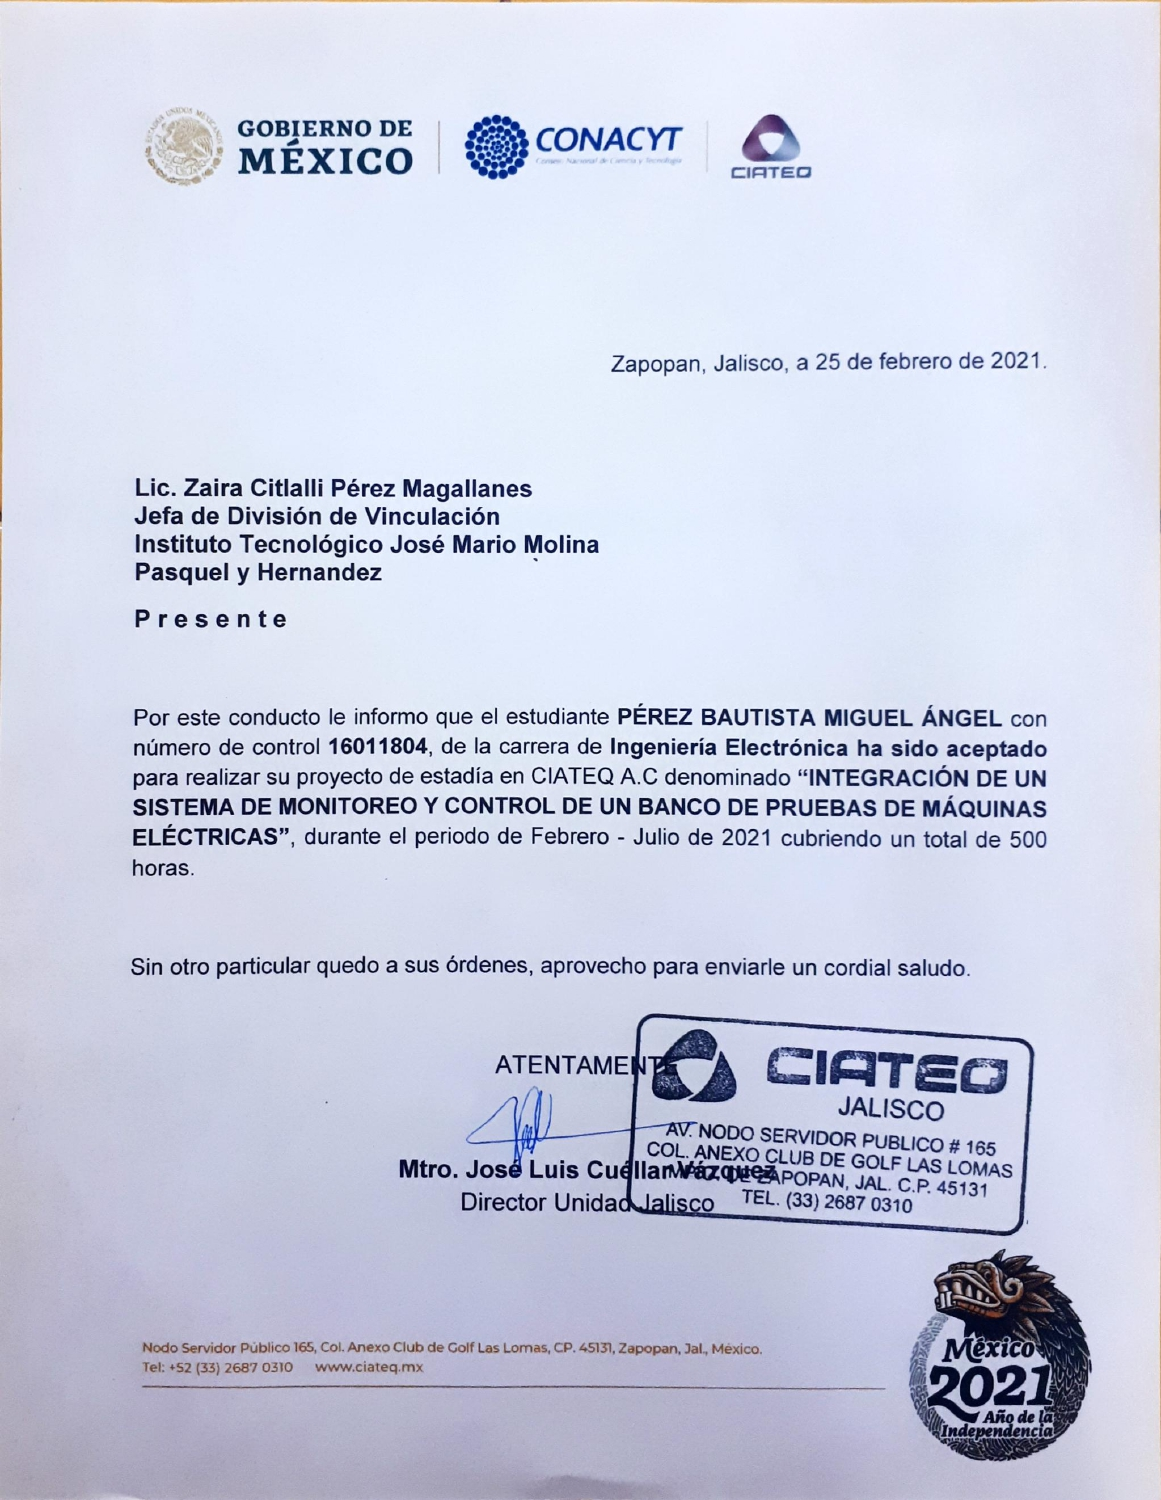
\includegraphics[scale=0.82]{carta_acep}
\caption{Carta de aceptación residencia profesional}
\end{figure}

\newpage
\section{Carta de finalización}

\newpage

\section{Introducción} %ligera introducción al tema y ligero hablar del proyecto

\iffalse
En las últimas decadas, los motores eléctricos se han convertido cada vez más en un elemento cotidiano para toda la población. Se presentan en una amplia variedad de aplicaciones pasando del uso generalmente en la industria para encontrarlos en los hogares, además de aplicaciones remotas de investigación en tierra, en el aire, en el agua y, finalmente, en el espacio, cada uno con sus propias características y protecciones específicas. \\[2.5mm]
Los motores se utilizan en muchas áreas como la robótica movil, brazos robóticos industriales, elevadores, grúas, taladros, autos eléctricos, drones o en otras aplicaciones de menores exigencias desde el punto de vista de control automático como bombas, bandas transportadoras, entre otros. \\[0.8mm]
\fi

Una máquina eléctrica es un dispositivo capaz de transformar cualquier forma de energía en energía eléctrica o viceversa, y también se incluyen en esta definición las máquinas que transforman la energía eléctrica en la misma forma de energía pero de una forma diferente que resulta más cómoda de transportar o utilizar.  \\[0.15mm]

Por lo tanto, la utilidad  de las máquinas eléctricas es indiscutible en la sociedad moderna desde dos vertientes; por un lado, los motores eléctricos constituyen el músculo de un sinmúmero de actividades industriales y domésticas. Por el otro, los generadores eléctricos aparecen casi en todas las formas de generación de energía elétrica.\\[0.15mm]

Los generadores transforman la energía mecánica en energía eléctrica, mientras que los motores transforman la energía eléctrica en energía mecánica girando en un eje. El motor se puede clasificar de corriente continua o motor de corriente alterna. Los transformadores y convertidores conservan la forma de la energía pero transforman sus características. \\[0.15mm]

Con este avance industrial, las máquinas eléctricas comenzaron a tomar un papel importante a lo largo del tiempo en el campo industrial, se comenzó a generar electricidad a gran escala usando generadores y se dio inicio a la distribución de la electricidad desde el pueblo más chico hasta las grandes ciudades. 
Se comenzó a dar un nuevo giro a la forma de vivir de cada habitante sobre la tierra conforme la electricidad llegaba a sus viviendas y lugares de trabajo, puesto que ahora con electricidad se daba  el inicio del desarrollo de dispositivos que funcionaran con electricidad, tal es el caso del bombillo, que una vez que su desarrollo fue completo, la vida de velas y antorchas quedó atrás en la historia de la humanidad. \\[0.8mm] 

Tal como pasó con los generadores de electricidad, también sucedió lo mismo para el motor eléctrico, dando paso al avance industrial para generar mayor trabajo mecánico usando una conversión de energía eléctrica a mecánica. El campo industrial comenzó a crecer exponencialmente, ya que tareas que para un humano eran difíciles de lograr, ahora para una máquina eléctrica a través de ejes de distribución de energía, engranes, poleas y cadenas, se lograba generar un trabajo mecánico eficiente y de mayor potencia, para lograr trabajos nunca antes vistos en aquella época. \\[0.15mm]

Es por ello que desde aquel punto en la historia, hasta la fecha, hablar de máquinas eléctricas es un tema importante en el área de ingeniería y desarrollo de tecnología, ya que hoy en día se sigue investigando para lograr que las máquinas eléctricas sean mejores, tanto en un mejor rendimiento de potencia y eficiencia, como también usando la menor energía posible que a su vez contribuya al cuidado del medio ambiente.  A nivel global se están llevando a cabo estudios para la mejora de estos dispositivos. \\[0.3mm]


\newpage
\section{Justificación}

Actualmente, investigadores del CIATEQ Jalisco  se encuentran trabajando en el estudio e investigación de las máquinas eléctricas, por lo cual surge la necesidad de desarrollar un banco de pruebas para motores y generadores eléctricos, donde se permita al investigador de CIATEQ recolectar datos de respuesta y comportamiento.\\

De esta manera, los investigadores del CIATEQ Jalisco tendrán al alcancé una mesa de pruebas, donde se podrá obtener la información de respuesta que necesiten, documentarla y así poder llegar  a nuevos desarrollos innovadores para máquinas eléctricas en el futuro. \\

\newpage 
\section{Objetivos}
A continuación se define el objetivo general y objetivos específicos del proyecto de residencia profesional. 
%Como en cualquier proyecto, se tiene dos tipo de objetivo, el objetivo general y los objetivos especificos. \\[0.8mm]
\subsection{Objetivo General}
El objetivo general del proyecto es el desarrollar e integrar un sistema de monitoreo y control que permita a los investigadores de CIATEQ Zapopan ejecutar pruebas a máquinas eléctricas dando uso a los actuadores de control y sensores de una manera dinámica e interactiva a través de una aplicación de escritorio, logrando así un banco de pruebas a máquinas eléctricas automatizado \\[0.8mm]

\subsection{Objetivos específicos}
Los objetivos específicos son los siguientes: \\[0.8mm]

\begin{itemize}
\item Identificar y conocer dispositivos del sistema (banco de pruebas).
\item Crear diagrama de bloques del sistema.
\item Identificar comunicaciones a usar. 
\item Tomar lectura del manual servomotor Kollmorgen.
\item Tomar lectura de comunicación Modbus.
\item Identificar comandos modbus del servomotor Kollmorgen.
\item hacer pruebas de comunicación Servomotor - PC.
\item Analizar que plataforma de Hardware será usada como controlador (Arduino Mega, Rpi).
\item Analizar que plataforma de desarrollo Software  será usada para HMI/Aplicación.
\item Realizar pruebas de control de dispositivos por medio del controlador. 
\item Comenzar con el desarrollo del programa de control del banco de pruebas.
\item Comenzar con el desarrollo del programa de software (HMI/Aplicación).
\item Versionado de desarrollo tanto del control como software.  
\item Desarrollo, pruebas y depuración entre programa de control y programa de software.
\item Hacer integración completa entre control y software. 
\end{itemize}
\newpage
\section{Caracterización del lugar de trabajo}
\begin{figure}[htbp]
\hspace*{-.15cm} 
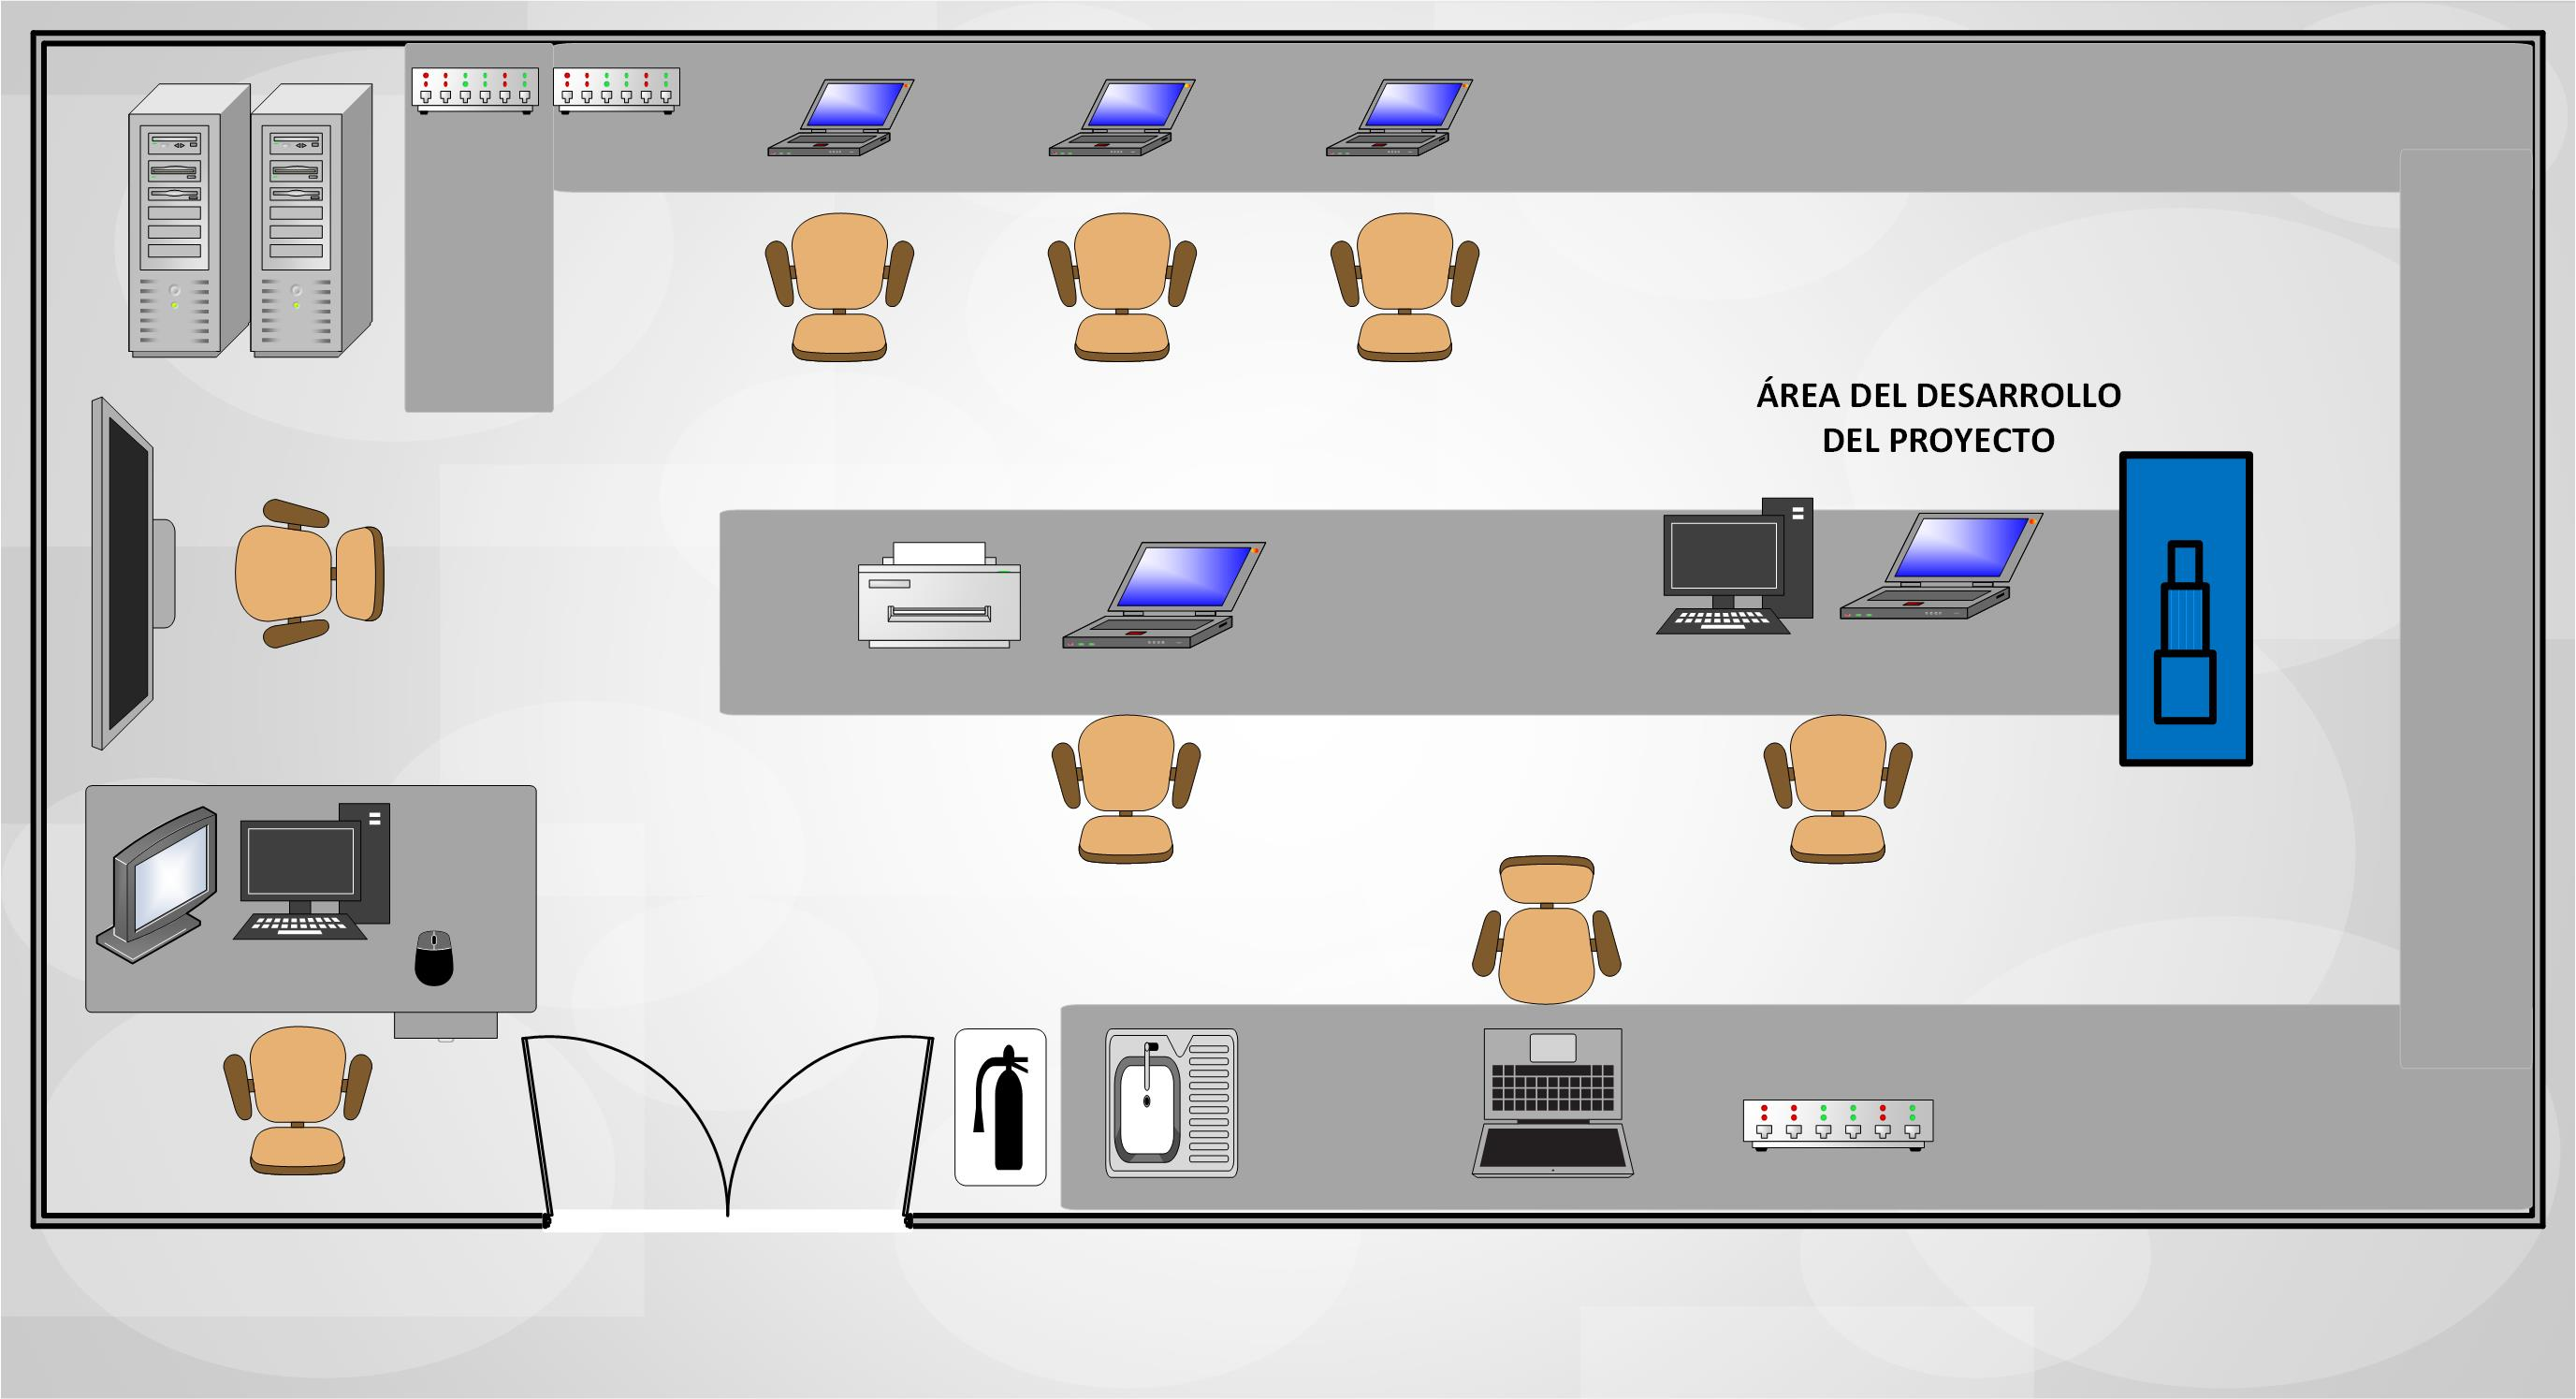
\includegraphics[scale=0.245]{lab2}
\caption{Plano del laboratorio de eficiencia energética CIATEQ Zapopan }
\end{figure}
\newpage
\section{Alcances y limitaciones de proyecto}
El alcance del proyecto debe de permitir un buen desarrollo de programa funcional, tanto del controlador como el programa del software (interfaz de usuario), se pretende llegar a ese punto donde se pueda ingresar a los dos modos de operación del sistema y poder realizar movimientos del servomotor (en el caso del modo generador) y obtener información de sensores desplegada en el interfaz de usuario. \\[2.5mm]
Por el lado del modo motor, se pretende el tomar datos de sensores y que sean visualizados de igual manera en la interfaz de usuario. \\[0.1mm]

%Como se observa se habla de dos modos de operación, donde por un lado  el servomotor kollmorgen se encuentra habilitado y los %sensores del sistema, y por el otro lado se inhabilita servomotor Kollmorgen y únicamente se encuentran los sensores %habilitados. \\[0.8mm]


Las limitación del proyecto es el tiempo que se ha dado para desarrollar la residencia profesional, ya que se comienza de cero este proyecto y se debe de dedicar tiempo en lectura, pruebas y desarrollo, así como también tiempo a dedicar para la depuración de errores que surjan en los programas. \\[0.8mm]

Por esta limitación se pretende llegar por lo menos a tener un programa de control y de software estructurados,  donde el modo generador este funcionando, que se ejecute algún movimiento de servomotor y se obtengan los respectivos datos de interés. \\[2.5mm]
Si existe la posibilidad de alargar fechas de entrega en residencia profesional, será posible tener también el modo motor en el sistema y completar la integración control - software. \\

\newpage
\section{Fundamento teórico}
En esta sección se desglosan los temas teóricos para llevar a cabo el proyecto de residencia. \\
\subsection{Sistemas embebidos}
Un sistema embebido es un sistema de computación diseñado para realizar algunas funciones dedicadas, frecuentemente en un sistema de computación en tiempo real. Al contrario de lo que ocurre con los ordenadores de propósito general (como por ejemplo una computadora personal o PC) que están diseñados para cubrir una amplia gama de necesidades, los sistemas embebidos se diseñan para cubrir necesidades especificas. \\[2.5mm] En un sistema embebido la mayoría de los componentes se encuentran incluidos en una placa base (tarjeta de vídeo, audio, módem, etc) y muchas veces los dispositivos resultantes no tiene el aspecto de lo que se suele asociar a una computadora. \\[2.8mm] Algunos ejemplos de sistemas embebidos podrían ser dispositivos como un taxímetro, un sistema de control de acceso, la electrónica que controla una máquina expendedora o el sistema de control de una fotocopiadora entre otras múltiples aplicaciones. \\[2.8mm]

Por lo general los sistemas embebidos se pueden programar directamente en el lenguaje ensamblador del microcontrolador o microprocesador incorporado sobre el mismo, o también, utilizando los compiladores específicos, pueden utilizarse lenguajes como C o C++,  en algunos casos, cuando el tiempo de respuesta de una aplicación no es factor crítico, también pueden usarse lenguajes Orientados a Objetos como JAVA.  \\[2.8mm]

Los programas de sistemas embebidos se enfrentan normalmente a tareas de procesamiento en tiempo real. \\[2.8mm]
Existen también plataformas desarrolladas por distintos fabricantes que proporcionan herramientas para el desarrollo y diseño de aplicaciones y prototipos con sistemas embebidos desde ambientes gráficos, algunos ejemplos de estas son: Arduino, mbed, Raspberry Pi, BeagleBone, Esp32, entre otros. 
\subsubsection{Componentes de un sistema embebido}
En la parte central se encuentra el microprocesador, microcontrolador, DSP, etc. Es decir, la CPU o unidad que aporta capaacidad de cómputo al sistema, pudiendo incluir memoria interna o externa, un micro con arquitectura específica según los requisitos.\\[2.8mm]
La comunicación adquiere gran importancia en los sistemas embebidos. Lo normal es que el sistema pueda comunicarse mediante interfaces estándar de cable o inalámbricas. Así un sistema embebido incorporará puertos de comunicaciones del tipo RS-232, RS-485, SPI, I2C, CAN, USB, WiFi, GSM, etc. \\[9.8mm]

El subsistema de presentación o representación gráfica suele ser una pantalla HMI, tactil, LCD, de segmentos, etc. \\[1.2mm]

Se denominan actuadores a los posibles elementos electrónicos que el sistema se encarga de controlar. Puede ser un motor eléctrico, un conmutador tipo relé, etc. El mas habitual puede ser una salida de señal PWM para control de la velocidad de motores de corriente continua. \\[0.8mm]

El módulo de E/S analógicas y digitales suele emplearse para digitalizar señales analógicas procedentes de sensores, activar diodos led, reconocer el estado abierto cerrado de un conmutador o un pulsador, etc. \\[0.8mm]

El módulo de reloj es el encargado de generar las diferentes señales de reloj a partir de un único oscilador principal. El tipo de oscilador es importante por varios aspectos: por la frecuencia necesaria, por la estabilidad necesaria y por el consumo de corriente requerido. El oscilador con mejores características en cuanto a estabilidad y coste son los basados en resonador de cristal de cuarzo, mientras que los que requieren menor consumo son los RC. Mediante sistemas PLL se obtienen otras frecuencias con la misma estabilidad que el oscilador patrón.\\[0.8mm]

El módulo de energía, se encarga de generar diferentes tensiones y corrientes necesarias para alimentar los diferentes circuitos del sistema. Usualmente se trabaja con un rango de posibles tensiones de entrada que mediante conversores ac/dc o dc/dc se obtienen las diferentes tensiones necesarias para alimentar los diversos componentes activos del circuito. \\[0.8mm]

Además de los conversores AC/DC, DC/DC, otros módulos típicos son; filtros, circuitos integrados, supervisores de alimentación, etc. \\ [0.8mm]
el consumo de energía puede ser determinante en el desarrollo de algunos sistemas embebidos que necesariamente se alimentan con baterías, con lo que el tiempo de uso del sistema suele ser la duración de la carga de las baterías.\\[2.8mm]

Como se puede observar con la información antes presentada, un sistema embebido es un circuito diseñado para un propósito específico, quiere decir que este circuito se le puede encomendar tareas especificas para que las realice. Regularmente cuando se habla de sistemas embebidos se habla de microprocesadores y microcontroladores, que son pieza fundamental en cualquier sistema embebido en el que se planea desarrollar.\\[0.8mm]

Se habla de sistemas embebidos en esta sección ya que es la parte inicial de cualquier sistema de control sea industrial o sea orientado a un placa de desarrollo de prototipos e investigación. \\[0.8mm]

Por lo tanto, un sistema de control es un sistema embebido en el cual cuenta con lo necesario para poder programar tareas que se necesite que el sistema realice por nosotros, por ejemplo con un sistema de control podríamos desarrollar un programa de control que nos ayude a monitorear la cantidad de luz que tenga un cierto cuarto y se despliegue en una pantalla LCD. Otro ejemplo común sería el monitorear la temperatura y la humedad de algún jardín. Todo esto se logra dando uso de un sistema de control, que por ende es un sistema embebido. \\[0.8mm]

\subsubsection{Arduino}
Arduino es una plataforma de desarrollo basada en una placa electrónica de hardware libre que incorpora un microcontrolador y una serie de pines como E/S digitales y analógicas. Estos permiten establecer conexiones entre el microcontrolador y los diferentes sensores y actuadores de una manera muy sencilla (principalmente con cables dupont)\\[0.8mm]

Una placa electrónica es una PCB (Printed Circuit Board, placa de circuito impreso). Las PCB son superficies planas fabricadas en un material no conductor, la cual costa de distintas capas de material conductor. Una PCB es la forma más compacta y estable para construir un circuito electrónico. Por lo tanto, la placa Arduino no es más que una PCB que implementa un determinado diseño de circuitería interna. De esta forma el usuario final no se debe de preocupar por las conexiones eléctricas que necesita el microcontrolador para funcionar, y puede empezar directamente a desarrollar las diferentes aplicaciones electrónicas que necesite. \\[0.8mm]

Cuando hablamos de arduino, deberíamos de especificar el modelo concreto. Se han fabricado diferentes modelos de placas Arduino oficiales, cada una pensada como un propósito diferente y características variadas (como el tamaño físico, número de pines E/S, modelo del microcontrolador, etc). A pesar de las varias placas que existen todas pertenecen a la misma familia (microcontroladores AVR marca Atmel). Esto significa que comparten la mayoría de sus características de software, como arquitectura, librerías y documentación. \\[0.8mm] 

El microcontrolador que lleva la placa de Arduino Uno es el modelo Atmega328P. La "P" del final significa que este chip incorpora la tecnología "Picopower"(propietaria de Atmel) y permite un consumo eléctrico ligeramente menor comparándolo con el modelo equivalente sin "Picopower", Atmega328 (sin la P). Aunque el Atmega328P puede trabajar a un voltaje menor y consumir menos corriente que el Atmega328, ambos modelos son funcionalmente idénticos , es decir, pueden ser remplazados el uno por el otro. \\[0.8mm]

\begin{figure}[htbp]
\hspace*{4.0cm} 
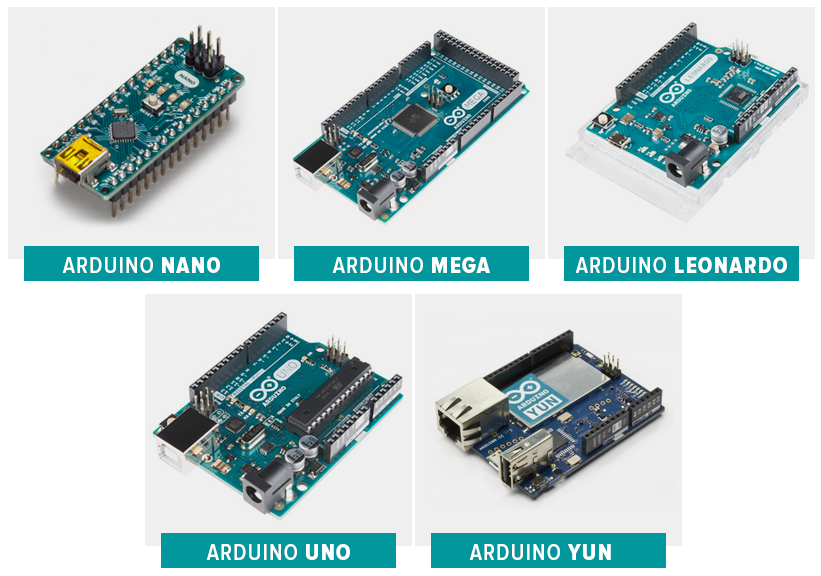
\includegraphics[scale=0.35]{arduino-familia}
\caption{Familia Arduino}
\end{figure}
\newpage
\subsubsection{Raspberry Pi}
Las Raspberry PI es una computadora de bajo costo y con un tamaño compacto, del tamaño de una tarjeta de crédito, puede ser conectactada a un monitor o a un TV y usarse con un mouse y teclado estándar. Es un pequeño computador que corre un sistema operativo linux capaz de permitirle a las personas de todas las edades explorar la computación y aprender a programar lenguajes como scratch y Python. \\ 
Es capaz de hacer la mayoría de las tareas típicas de un computador de escritorio, desde navegar en internet, reproducir vídeos, manipular documentos y hasta reproducir juegos. \\[0.8mm]

Además la Rasberry Pi, tiene la habilidad de interactuar con el mundo exterior, puede ser usada en una amplia cantidad de proyectos digitales, desde reproductores de música y vídeo, detector de rostros, estaciones meteorológicas hasta cajas de aves con cámaras infrarrojas. \\[0.8mm]

Raspberry es muy usada por gente dedicada al desarrollo de software, desarrollo de aplicaciones, desarrollo de proyectos y prototipos. Además de que también entra en el área de la investigación e ingeniería donde con ayuda de plataformas y hardware externo se pueden realizar proyectos muy interesantes. \\[0.8mm]

Las Raspberry también es un sistema embebido, al igual que arduino, con la única diferencia de que el arduino es un microcontrolador que esta listo para recibir ordenes, y una Raspberry cuenta con un microprocesador el cual funciona más como una computadora, ya que a un arduino no es posible cargarle un sistema operativo y  una Raspberry PI si.\\ 

Lo interesante de la Raspberry es que tiene un sin fin de aplicaciones mayores a las de un arduino, por que se puede dar uso de Python, OpenCV, bases de datos MySQL además se tiene dentro del mismo hardware módulo bluetooth y Ethernet, entre otros.\\ 

Recursos que arduino no tiene, por lo tanto Raspberry es una buena opción si tu proyecto requiere dar uso a los recursos de harware que Rpi tiene embebidos en su placa. \\[0.8mm]

Algunas de sus especificaciones técnicas que tiene Raspberry PI 3 B+  se tienen en la siguiente imagen: \\ 

\begin{figure}[htbp]
\hspace*{2.2cm} 
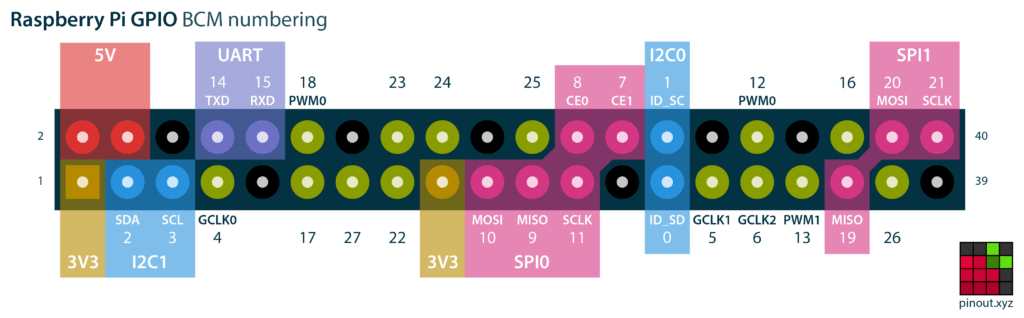
\includegraphics[scale=0.42]{GPIO_RPI}
\caption{Pinout GPIO Raspberry Pi 3 B+}
\end{figure}
\newpage
La Raspberry Pi 3 B+ cuenta con un GPIO de 40 pines, el cual permite el contacto con el mundo exterior, tanto por sensores como actuadores, en este punto es importante conocer que el GPIO de Raspberry trabaja con un nivel de 3.3 V, así que si quieres conectar sensores que operan a 5V necesitarás un conversor de niveles lógicos, el cual se recomienda el MCI00582 que es comercializado por MCI Electronics. \\

Debido que el procesador de la Raspberry Pi no tiene un conversor analógico a digital embebido, y si se requiere leer sensores analógicos se debe de dar uso a un conversor ADC externo, el cual el que recomienda el fabricante es el MCI01856. 
Rpi además cuenta con puertos de comunicación I2C, SPI y UART. \\[0.8mm] 

La Raspberry Pi 3B+ cuenta con conexiones tradicionales como son puertos USB,  conector de red ethernet, jack de 3.5 mm , puerto HDMI, puerto para memoria microSD y un conector micro-usb para alimentación. También se destacan los puertos especiales para la cámara y la pantalla. \\ \\ [0.8mm] 

\begin{figure}[htbp]
\hspace*{3.8cm} 
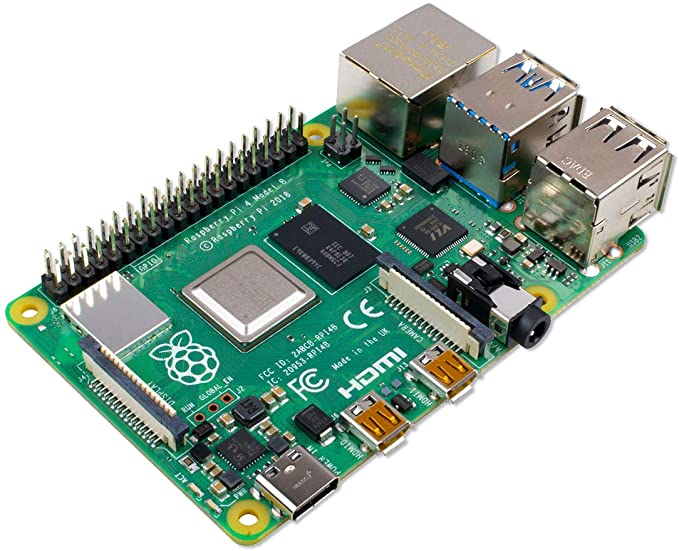
\includegraphics[scale=0.42]{Rpi}
\caption{Raspberry Pi 3 B+}
\end{figure}

\newpage
\subsubsection{ESP32}
ESP32 es una serie de SoC (System on Chip) y módulos de bajo costo y bajo consumo de energía creado por Espressif Systems. \\

Esta nueva familia es la sucesora del conocido ESP8266 y su características más notable es que, además de WiFi, también soporta Bluetooth.
ESP32 se basan en un microprocesador Tensilica Xtensa LX6 (De uno o dos nucleos) con una frecuencia de operación de hasta 240 Mhz. \\

Los ESP32 poseen un alto nivel de integración, en su pequeño encapsulado incluyen: 

\begin{figure}[htbp]
\hspace*{0.5cm} 
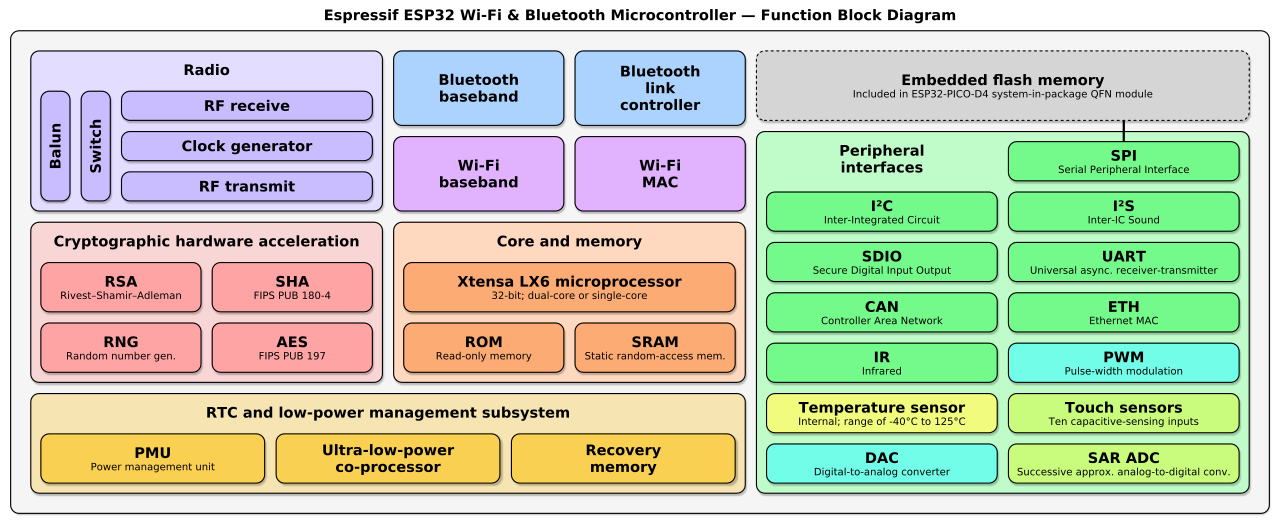
\includegraphics[scale=0.38]{especi_32}
\caption{Diagrama de bloques de funciones de ESP32}
\end{figure}

Además  logra un consumo de energía muy bajo a través de funciones de ahorro de energía que incluyen sincronización de reloj y múltiples modos de operación. Todo esto lo convierte en la herramienta ideal para tus proyectos energizados con baterias o aplicaciones IoT. \\[0.8em]

Este sistema embebido tiene gran robustez para el desarrollo de aplicaciones de media y  gran escala, cuenta con el hardware y potencia necesaria para llevar a cabo tus proyectos a otro nivel. \\[0.8mm] 

\begin{figure}[htbp]
\hspace*{5.5cm} 
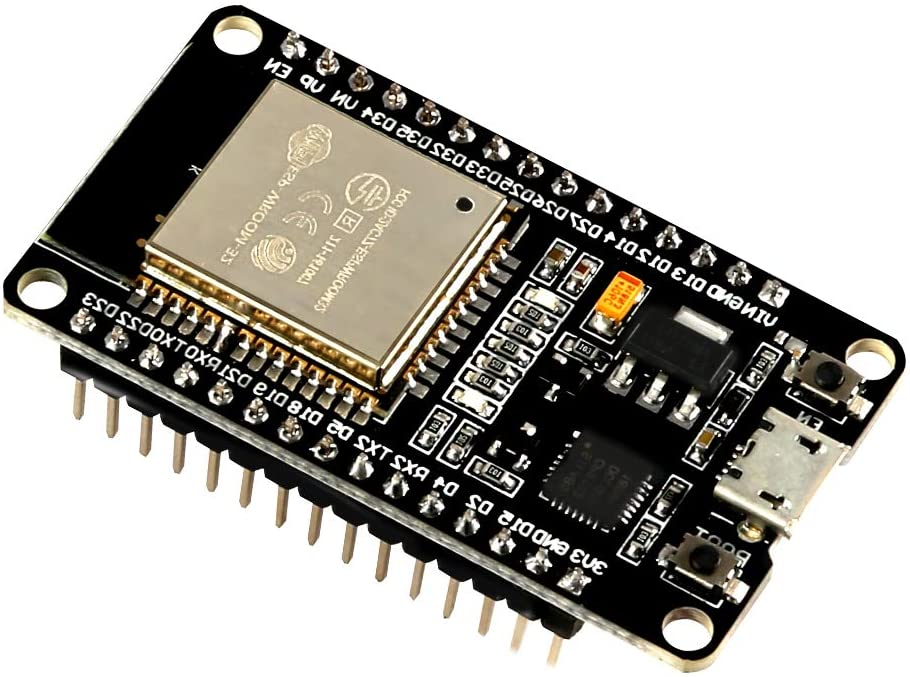
\includegraphics[scale=0.20]{ESP-32}
\caption{ESP-32}
\end{figure}

\newpage
\subsection{Sensores Industriales}
Para poder controlar automáticamente un proceso de fabricación es necesario disponer de información sobre el estado del proceso. Esto se puede hacer midiendo diferentes magnitudes físicas que intervienen en el mismo. Pese a poder recibir diferentes nombres (detector, transductor, sonda), el sensor es el nombre más utilizado en control de autómatas para referirse al dispositivo que mide una magnitud física. \\

En general estas magnitudes físicas no tienen por que ser eléctricas, por lo que se utilizan transductores para convertir a señales eléctricas. \\[0.8mm]

Un transductor convierte una señal no eléctrica en eléctrica, en la cual alguno de sus parámetros (nivel de tensión, corriente, frecuencia) contiene información sobre la magnitud de medida. \\ Puesto a que es necesario acoplar la salida de este dispositivo transductor al sistema de control, puede ser necesario efectuar filtrado y amplificación de la señal eléctrica en el llamado circuito acondicionador o de acondicionamiento. \\[0.8mm] 

En esta sección se hablará de los sensores de encoder, de velocidad y torque. \\ 
\subsubsection{Encoder}
El encoder es un transductor rotativo, que mediante una señal eléctrica sirve para indicar la posición angular de un eje, velocidad y aceleración del rotor de un motor. \\[0.8mm]

\paragraph{Funcionamiento}\leavevmode\newline 
Un encoder se compone básicamente de un disco conectado a un eje giratorio.\\
El disco esta hecho de vidrio o plástico y se encuentra 'codificado' con unas partes transparentes y otras opacas que bloquean el paso de luz emitida por la fuente de luz (típicamente emisores infrarrojos). En la mayoría de los casos, estas áreas bloqueadas (codificadas) están arregladas en forma radial. \\[0.8mm] 

A medida que el eje rota, el emisor infrarojo emite luz que es recibida por el sensor óptico (o foto-transistor) generando los pulsos digitales a medida que la luz cruza a través del disco o es bloqueada en diferentes secciones de este. \\[0.8mm]
Esto produce una secuencia que puede ser usada para controlar el radio de giro, la dirección del movimiento e incluso la velocidad. 
\newpage

\begin{figure}[htbp]
\hspace*{3.5cm} 
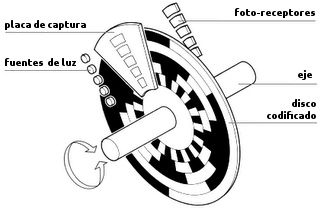
\includegraphics[scale=0.75]{partes-encoder}
\caption{Partes de un encoder}
\end{figure}

\paragraph{Tipos de encoder}\leavevmode\newline
Una clasificación de los encoder según el tipo de información sobre la posición que genera sería: \\[0.8mm]

\textbf{Incremental}
Como su nombre lo indica, es un encoder que determina el ángulo de posición por medio de realizar cuentas incrementales. \\
Esto quiere decir que el encoder incremental provee una posición estratégica desde donde siempre comenzará la cuenta. La posición actual del encoder es incremental cuando es comparada con la última posición registrada por el sensor. \\

Los encoders incrementales son un tipo de encoder óptico y este en este tipo de encoder cada posición es completamente única. 
Un encoder incremental típico es el encoder de cuadratura. \\[0.8mm]


Corresponde a un tipo de encoder incremental que utiliza dos sensores ópticos posicionados con un desplazamiento de $\frac{1}{4}$ de ranura el uno del otro, generando dos señales de pulsos digitales desfasadas en $90^{\circ}$ o en cuadratura. A estas señales de salida, se les llama comúnmente A y B. Mediante ellas es posible suministrar los datos de posición, velocidad y dirección del eje. Si se incluye la señal de referencia, se le denomina I (índice). \\[0.8mm]

Usualmente, si la señal A adelanta a la señal B (la señal A toma valor lógico '1' antes que la señal B, por ejemplo), se establece el convenio de que el eje está rotando en sentido horario, mientras que si B adelanta a A, el sentido será antihorario.\\

\textbf{Absoluto}
Se basa en la información proveída para determinar la posición absoluta en secuencia. Un encoder absoluto ofrece un código único para cada posición. \\

Se dividen en dos grupos: los encoders de un solo giro y los encoders absolutos de giro múltiple. \\
\newpage

\textbf{Monovuelta}
Dividen una revolución mecánica en un número determinado de pasos de medición. Tras una revolución completa, los valores de medición se repiten. El número máximo de pasos es de 8.192 \\[0.8mm] 

\textbf{Multivuelta}
No sólo registran la posición angular, sino que también cuentan las revoluciones (hasta un máximo de 4.096). La emisión de las señales se efectúa ya sea a través de una interfaz SSI o de un sistema de bus tipo CAN o Profibus. \\[0.8mm] 

\subsubsection{Sensor de par y torsión}
Los sensores de par y torsión miden la fuerza de torsión a la que se somente un eje durante las diferentes fases de su funcionamiento, bien sea en arranque, dinámico o parada. \\[0.8mm] 

Estos sensores de par y torsión se utilizan para ensayar y estudiar elementos de rotación como motores, generadores, alternadores, entre otros. También hay sensores de par estático que miden la torsión o par sin que exista rotación, por ejemplo en una llave dinamométrica.\\[0.8mm] 

Un transductor de par proporciona una variación mecánica en una eléctrica, en este caso una torsión se traduce en una variación de voltaje. \\[0.8mm] 

Los tipos de sensores de par y torsión son diferentes, pero por tecnología se dividen en estáticos o dinámicos, a su vez, estos últimos se dividen en sensores de par dinámicos sin escobillas o anillos rozantes y sensores de par con escobillas o anillos rozantes.\\[0.8mm] 

Los formatos son variados, aunque siempre hay un denominador común, consta de un eje instrumentado,  que ha de ser intercalado entre la fuente y carga, para que el sensor de par, sea sometido a la torsión que deseamos medir. \\[0.8mm] 

\begin{figure}[htbp]
\hspace*{4.5cm} 
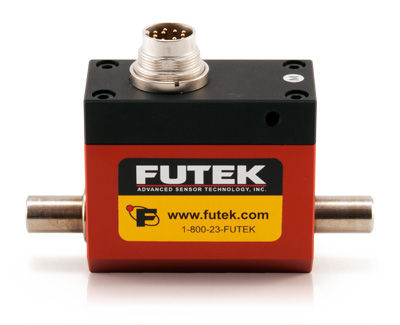
\includegraphics[scale=0.80]{sensor_futek}
\caption{Sensor de torque Futek}
\end{figure}
\newpage
\paragraph{Sensores de reacción}\leavevmode\newline
Los sensores de reacción utilizan galgas extensiométricas en configuración de puente completo con partes inmóviles que no requieren mantenimiento.  Pueden ser usados para comprobar el torque residual en sujetadores y determinar el torque para vencer los efectos de la fricción. \\[0.8mm] 
Su principal diferencia radica en que este tipo de sensores no gira su eje. \\ \\

\begin{figure}[htbp]
\hspace*{5.0cm} 
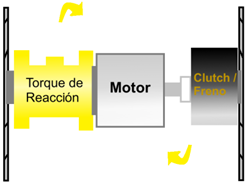
\includegraphics[scale=0.79]{reaccion_sens}
\caption{Sensor de reacción}
\end{figure}

\paragraph{Sensores de torque rotatorios}\leavevmode\newline
Los sensores de torque rotatorios ofrecen ventajas para realizar mediciones en el desempeño de herramientas y maquinaria. Se ofrecen configuraciones de montaje sin contacto y son capaces de detectar el torque dinámico en velocidades de hasta 12,000 RPM.\\[0.8mm] 

\begin{figure}[htbp]
\hspace*{4.6cm} 
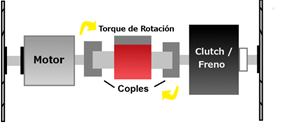
\includegraphics[scale=0.89]{rotatorio}
\caption{Sensor de torque rotatorio}
\end{figure}
\newpage
\paragraph{Rotatorios de contacto}\leavevmode\newline
En estos sensores giratorios los elementos de medición están conectados por medio de escobillas internas, lo que no permite velocidades altas. \\

Sus principales características son:
\begin{itemize}
\item Capacidad desde 10Nm hasta 10,000 Nm.
\item Velocidades hasta 3,000 RPM. \\
\end{itemize}
\begin{figure}[htbp]
\hspace*{4.6cm} 
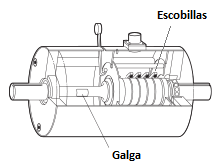
\includegraphics[scale=0.89]{contacto_sens}
\caption{Sensor del tipo rotatorio de contacto}
\end{figure}

\paragraph{Rotatorios de no contacto}\leavevmode\newline
En estos sensores giratorios la medición de torque se realiza por medios magnéticos, por lo que, al no tener elementos de contacto, permite velocidades más grandes y no hay desgaste de las escobillas. \\

Sus principales características son:
\begin{itemize}
\item Capacidad desde 10Nm hasta 10,000 Nm.
\item Velocidades hasta 12,000 RPM. \\
\end{itemize}

\begin{figure}[htbp]
\hspace*{5.6cm} 
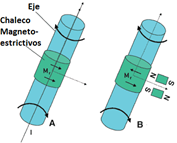
\includegraphics[scale=0.89]{no_contact_sens}
\caption{Sensor del tipo rotatorio de no contacto}
\end{figure}
\newpage
La avanzada tecnología de los sensores basados en galgas extensiométricas es ampliamente conocida en muchas áreas de la industria por poseer: \\

\begin{itemize}
\item Alta exactitud, la cual cumple con muchos estándares de calidad en la industria automotriz y aeroespacial.
\item Construcción robusta en acero inoxidable o aluminio para dar mayor resistencia. 
\item Garantía de fabricación para una larga duración incluso en las más rigurosas condiciones de trabajo. 
\item Una amplia variedad de opciones de montaje, tamaños y geometrías. 
\item Precio competitivo.
\item Amplia variedad de capacidades.
\item Alta respuesta frecuencial acoplada con diseños mecánicamente rígidos. 
\end{itemize}

Estos sensores de torque son empleados en muchas aplicaciones dentro de la industria tales como médica, automotriz, aviación, aeroespacial, computación y automatización, entre otras. 
\subsection{Protocolos de comunicación industrial}
Un protocolo de comunicación industrial son un conjunto de reglas que permiten las interferencias e intercambios de datos entre varios dispositivos que forman una red. \\

A medida que la tecnología ha avanzado, estos van teniendo un proceso de evolución, las comunicaciones a este nivel debe de poseer unas características particulares para responder a las necesidades de intercomunicación en tiempo real. Los protocolos que se usan en la industria provienen, por un lado, de la evolución de los antiguos protocolos basados en comunicaciones serie,y, por otro lado, de la creación de nuevos estándares basados en nuevas tecnologías. Como ejemplo de evolución de los antiguos protocolos se pueden citar Modbus/TCP, DNP3, Profinet, etc. \\

Estos protocolos se aprovechan de las ventajas funcionales y de seguridad que ofrecen tanto Ethernet como TCP/IP  para ofrecer mejores capacidades de transferencia de información en los sistemas de control. Así, la mayoría de ellos se basan en encajar la parte de datos del protocolo original en la parte de datos de una trama Ethernet. \\ 

Basa en los protocolos estándar TCP/IP, utiliza ya los bastantes conocidos hardware y software ethernet para establecer un nivel de protocolo para configurar, acceder y controlar dispositivos de automatización industrial. Ethernet/IP clasifica los nodos de acuerdo a los tipos de dispositivos preestablecidos, con sus actuaciones específicas. Ethernet/IP ofrece un sistema integrado completo, enterizo, desde la plana industrial hasta la red central de la empresa. \\

Uno de los objetivos principales del Ethernet/IP es que utiliza todas sus herramientas y tecnologías tradicionales, como los son los protocolos de transporte (TCP), Internet(IP) y las tecnologías de acceso y señalización de medios que se encuentran dentro de las tarjetas de interfaz de Ethernet. \\ 

\newpage
\subsubsection{DeviceNet}
DeviceNet es un protocolo de comunicación  usado en la industria de la automatización para interconectar dispositivos de control para el intercambio de datos. Un protocolo de comunicación es el quien  permite que dispositivos individuales (arrancadores, sensores, escáner, motores, etc) comuniquen con el controlador de red. Una forma de verlo es que el término capa de aplicación implica que DeviceNet trata más con los datos de la aplicación que un nivel más bajo o un protocolo de capa que no es de aplicación. \\[0.8mm]

\begin{figure}[htbp]
\hspace*{5.6cm} 

\includegraphics[scale=0.89]{DeviceNet_Logo}
\caption{Logo DeviceNet}
\end{figure}
\vspace{8mm}
\subsubsection{Modbus TCP/IP}
El protocolo Modbus TCP/IP es un protocolo de comunicación diseñado para permitir a que equipos industriales tales como PLCs, PCs, drivers para motores y otros tipos de dispositivos físicos de entrada/salida puedan comunicarse sobre una red Ethernet, mientras que el Modbus RTU  es una representación binaria compacta de los datos adquiridos. El protocolo Modbus permite el control de una red de dispositivos, por ejemplo para que un equipo de medición de temperatura y humedad pueda comunicar los resultados a una computadora. Modbus también se usa para la conexión de un PC de supervisión con una unidad remota (RTU) en sistemas de supervisión de adquisición de datos (SCADA). \\ [0.8mm] 

\begin{figure}[htbp]
\hspace*{3.6cm} 
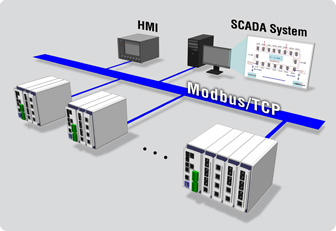
\includegraphics[scale=0.89]{red_modbus}
\caption{Red Modbus TCP/IP}
\end{figure}

\newpage

\subsubsection{PROFINET}
Profinet está basado en Ethernet industrial, TCP/IP y algunos estándares de comunicación pertenecientes al mundo TI. \\
Entre sus características destaca que es Ethernet en tiempo real, donde los dispositivos que se comunican por el bus de campo acuerdan cooperar en el procesamiento de solicitudes que se realizan dentro del bus. \\[0.7mm] 

Existen varios protocolos definidos dentro del contexto PROFINET como son: \\

\paragraph*{PROFINET/CBA:} Protocolo asociado a las aplicaciones de automatización distribuida en entornos industriales. 
\paragraph*{PROFINET/DCP:} Descubrimiento y configuración básica. Es un protocolo basado en la capa de enlace, utilizado para configurar nombres de dispositivos y direcciones IP. 
\paragraph*{PROFINET/IO:} A veces llamado PROFINET-RT(RealTime), es utilizado para comunicaciones con periferias descentralizadas.
\paragraph*{PROFINET/MRP:} Protocolo utilizado para la redundancia de medios. Utiliza los principios básicos para la reestructuración de las redes en caso de sufrir un fallo cuando la red posee la topología en anillo.
\paragraph*{PROFINET/MRRT:} Su objetivo es dar soluciones a la redundancia de medios para PROFINET/RT. 
\paragraph*{PROFINET/PTCP:} Protocolo de control de precisión de tiempo basado en la capa de enlace, para sincronizar señales de reloj/tiempo en varios PLC. 
\paragraph*{PROFINET/RT:} Transferencia de datos en tiempo real. 
\paragraph*{PROFINET/RT:} Transferencia de datos isócrono en tiempo real. \\ \\ 

\begin{figure}[htbp]
\hspace*{5.5cm} 

\includegraphics[scale=0.59]{profinet}
\caption{Logo de PROFINET}
\end{figure}
\newpage
\subsubsection{PROFIBUS}
Es un estándar de red de campo abierto e independiente de proveedores, donde la interfaz de ellos permite amplia aplicación de procesos, fabricación y automatización predial. \\[0.8mm] 
Profibus proporciona tres versiones diferentes de protocolos de comunicación: \\ \\

\paragraph*{Profibus-DP:} este protocolo está optimizado para conseguir una alta velocidad de transmisión. Está especialmente diseñado para establecer la comunicación entre el controlador programable (PLC) y los dispositivos de entrada/salida a nivel campo.  
\paragraph*{Profibus-PA:} está especialmente diseñada para conseguir una comunicación fiable a alta velocidad en ambientes expuestos a peligro de explosión.  
\paragraph*{Profibus-FMS:} se utiliza para la comunicación a nivel célula, donde lo principal es el volumen de información y no el tiempo de respuesta.\\

\begin{figure}[htbp]
\hspace*{6.0cm} 

\includegraphics[scale=0.25]{profibus}
\caption{Logo de Profibus}
\end{figure}
\newpage
\subsubsection{EtherCAT}
Es un protocolo de código abierto para informática y tiene alto rendimiento que pretende usar protocolos Ethernet en el ambiente industrial y es uno de los protocolos más rápidos en la actualidad. Por ejemplo, con el método de transmisión de EtherCat, el paquete de Ethernet se recibe, después es copiado en el dispositivo, se interpreta y se procesa. Los medios de EtherCAT encajan bien para los ambientes industriales o de control puesto que pueden ser accionado con o sin interruptores.\\
EtherCAT es un estándar abierto que se ha publicado como especificación del IEC basada en la entrada del grupo de la tecnología de EtherCAT. \\ \\
EtherCAT es especialmente adecuado para las aplicaciones rápidas. Entre las aplicaciones características se incluyen máquinas de embalar, máquinas de fundición y centros de mecanizado. \\[0.8mm]

Las capacidades de sincronización y utilización completa del ancho de banda son muy atractivas para aplicaciones de movimiento donde se requiere la sincronización de un gran número de unidades. Ahorra gastos de instalación al eliminar tanto la topología de  inicio de Ethernet como todos los conmutadores, enrutadores y concentradores.\\ 

EtherCAT encaja en el espectro de capas de aplicaciones de Ethernet donde el rendimiento, la topología y el costo general de implementación son factores determinantes. \\ 

\begin{figure}[htbp]
\hspace*{6.0cm} 
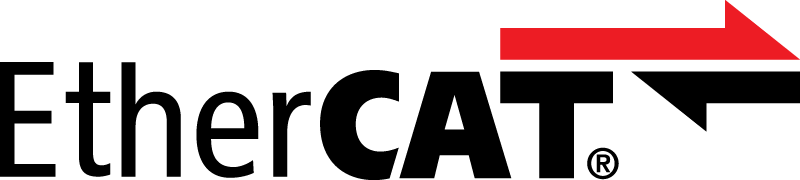
\includegraphics[scale=0.25]{ethercat}
\caption{Logo de EtherCAT}
\end{figure}
\newpage
\subsection{Interfaz gráfica de usuario}
La interfaz de gráfica de usuario o GUI (Graphic User Interface) es el entorno visual de imágenes y objetos mediante el cual una máquina y un usuario interactúan. A mediados de los años setenta, las GUI comenzaron a sustituir a las interfaces de línea de comandos, y esto permitió que la interacción con las computadoras fuera más sencilla e intuitiva. \\

En el campo de la ingeniería en mecatrónica las interfaces gráficas de usuario son parte fundamental de cualquier sistema desarrollado, ya que estas mismas son las que logran mantener una comunicación Humana - máquina y  poder observar la adquisición de datos del sistema, como por ejemplo los valores de estado de sensores y accionamiento de ciertos actuadores, entre otros. \\ 

\subsubsection{HMI (Human Machine Interface)}
Las HMI son las siglas de Human-Machine Interface, se refieren a un panel que permite a un usuario comunicarse con una máquina, software o sistema. Técnicamente, se puede referir a cualquier pantalla que se use para interactuar con un equipo, pero se utiliza normalmente para los entornos industriales. Las HMI muestran datos en tiempo real y permiten al usuario controlar con una interfaz gráfica de usuario \\ \\

En un entorno industrial, una HMI puede tener distintas formas. Puede ser una pantalla independiente, un panel acoplado a otro equipo o incluso una tablet. Da igual su aspecto; su uso principal es permitir a los usuarios visualizar los datos operativos y controlar las máquinas. Los operarios pueden usar una HMI como por ejemplo, ver qué  cintas transportadoras están encendidas  o ajustar la temperatura de un depósito de agua industrial. \\

\paragraph{Usos de la HMI}\leavevmode\newline
La HMI se utiliza en una amplia gama de sectores. Es común en la fabricación de distintos productos, desde automóviles, comida y bebidas y medicina. Industrias como la de la energía, el agua, las aguas residuales, los edificios y el transporte también pueden usar HMI. Cargos como los integradores de sistemas, operarios e ingenieros y, en espacial, los ingenieros en sistemas de control de procesos, usan frecuentemente HMI para controlar máquinas, platas o edificios. \\[0.8mm] 

La sofisticación de la HMI varía en función de la complejidad de la máquina o sistema para el que se usa. También varía según el uso de la HMI, ya sea para supervisar una máquina o para otros fines, como supervisar operaciones de una planta y controlar equipos. \\ 

Cuando el sistema de supervisión, control y adquisición de datos (SCADA)se comunica con los controladores lógicos programables (PLC) y los sensores de entrada/salida para obtener información sobre el funcionamiento de los equipos, esa información se muestra en una HMI, ya sea en un gráfico, gráfica u otra representación visual que sea fácil de leer y entender. Con una HMI, podrá ver toda la información de rendimiento de los equipos de una instalación en un solo lugar, mejorando la visibilidad de las operaciones de la planta.  Los operarios también pueden ver y gestionar las alarmas con una HMI asegurando que se puedan tratar rápidamente. 
\newpage

Los operarios también pueden controlar los equipos con las HMI para aumentar la productividad o adaptarse a las circunstancias cambiantes. Pueden hacer ajustes basados en los datos que ven en la HMI, haciendo que este proceso sea más rápido y sencillo. \\

A medida que el Internet de las Cosas (IoT) sigue desempeñando un importante papel en las instalaciones industriales, las HMI se vuelven más útiles. Pueden usarlas para visualizar datos y controlar los distintos equipos conectados de sus instalaciones. \\

\paragraph{HMI y SCADA}\leavevmode\newline
 HMI y SCADA se confunden por sus similudes y por que trabajan juntos. La mayoría de veces la HMI forma parte de un sistema SCADA.\\
 
Un sistema SCADA se utiliza para controlar sistemas grandes, como una planta entera. Es una combinación de otros sistemas como PLCs, sensores y unidades de terminales remotas (RTU). Un sistema SCADA recopila y registra datos, y puede controlar las operaciones automáticamente. \\ 

Una HMI, por su parte, es una interfaz gráfica para interactuar con un sistema SCADA y otros sistemas y equipos. Ambos elementos esenciales de un sistema de control industrial más grande. Mientras que el SCADA recopila y almacena los datos, la HMI permite a los usuarios interactuar con los equipos y gestionarlos mediante un panel. Ambos son necesarios. Sin SCADA, una HMI no tendría información que mostrar ni podría controlar los equipos. Sin una HMI, los usuarios no podrían ver los datos que el sistema SCADA recopila ni decirle cómo controlar los equipos. \\ 

SCADA y HMI son partes de un sistema más grande. SCADA funciona en segundo plano mientras que la HMI es normalmente el único elemento con el que interactúan los usuarios. Por ello a veces se hace referencia a ellos conjuntamente. \\  

\paragraph{Ventajas de la HMI}\leavevmode\newline
Las HMI proporcionan una serie de ventajas en las organizaciones industriales tales como: 

\paragraph*{Mayor Visibilidad:} una HMI de alto rendimiento le ofrece una mayor visibilidad de sus operaciones en todo momento, lo que le permite ver el rendimiento de sus equipos o instalaciones desde un solo panel, al que puede acceder incluso remotamente, aumentando la productividad con el tiempo y respondiendo a las alertas con mayor rapidez.
 
\paragraph*{Eficiencia Mejorada:} gracias al acceso en tiempo real de la HMI a los datos, se puede usar para supervisar la producción y ajustarla a los requisitos cambiantes. La visualización de los datos, combinados con las tecnologías de análisis de datos, le permiten identificar áreas en las que puede mejorar la eficiencia de sus operaciones. 

\paragraph*{Menos periodos de inactividad:} con las alertas en un panel central puede responder a los problemas con más rapidez, reduciendo periodos de inactividad. Visualizar y analizar los datos de rendimiento de los equipos también le pueden ayudar a detectar futuros problemas mecánicos y atajarlos antes de que puedan provocar periodos de inactividad más significativos. 

\paragraph*{Usabilidad Mejorada:} las HMI facilitan a los usuarios ver y entender los datos y equipos de control. Presentan los datos en forma de gráficos, gráficas, etc. Permitiendo a los usuarios interpretarlos rápidamente.

\paragraph*{Sistema Unificado:} con las HMI puede controlar todos los equipos usando la misma plataforma, lo que facilita a los operarios su control. También puede ver todos los datos en una ubicación, para tener una visión general clara de las instalaciones. Además, todos los usuarios reciben actualizaciones en tiempo real, con lo que su equipo estará siempre en la misma página. 

\paragraph{El futuro de la HMI}\leavevmode\newline
A medida que los datos sumen un papel más importante en los procesos industriales, la HMI está llamada a ser aún más importante. La tecnología ha avanzado significativamente en los últimos años, pero seguirá evolucionando en el futuro. \\

Más empresas están cambiando a las HMI de alto rendimiento, que atraen la atención de los usuarios solo a la información más crítica, ayudándoles a dar sentido a todos los datos disponibles y evitando el exceso de información. Las empresas también usan cada vez más pantallas multitáctiles, supervisión remota y sistemas en la nube. \\

A medida que la tecnología evolucione, las empresas utilizarán más análisis de datos avanzados e inteligencia artificial para obtener más conocimientos, comunicándoselos a los usuarios a través de las HMI que , en el futuro, también incorporarán realidad aumentada (AR), superponiendo gráficos digitales sobre el mundo real, y tecnología de realidad virtual (VR), que sumerge a los usuarios a un mundo digital para proporcionarles información visual más efectiva. Como la automatización sigue desempeñando un papel más central en los procesos industriales, los usuarios pueden aprovechar las HMI para supervisar y ajustar las actividades automatizadas. 

\begin{figure}[htbp]
\hspace*{4.5cm} 
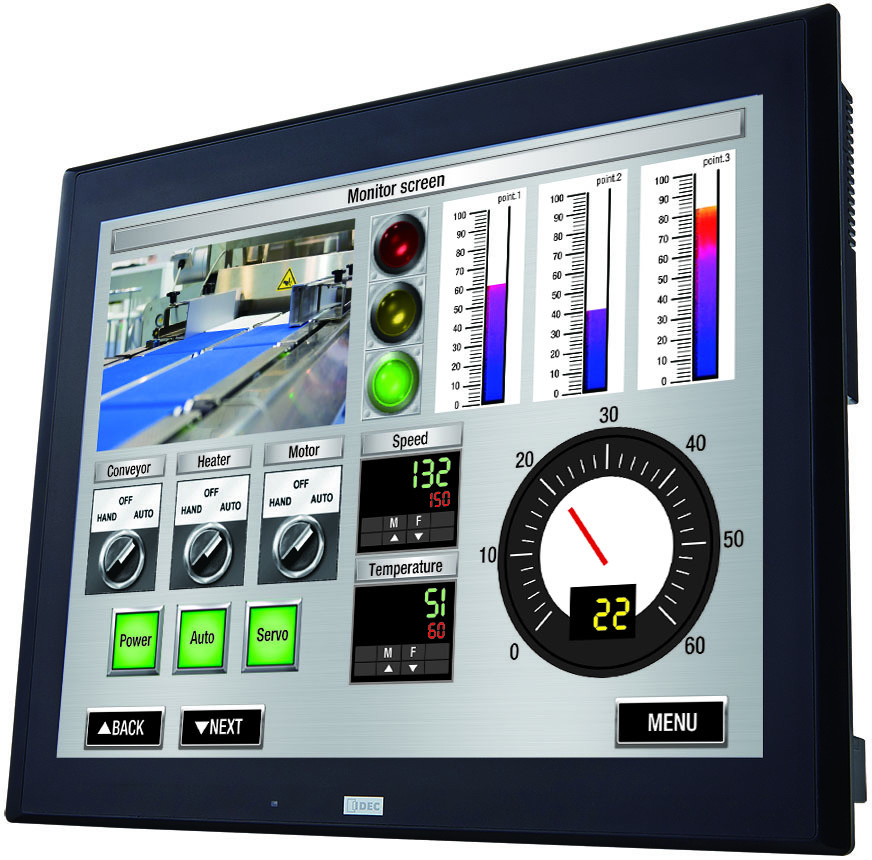
\includegraphics[scale=1.10]{HMI}
\caption{Ilustración de una HMI}
\end{figure}
\newpage

\subsection{Servomotores Industriales}
Un servomotor es un actuador rotativo o motor que permite un control preciso en términos de posición angular, aceleración y velocidad, capacidades que un motor normal no tiene. Utiliza un  motor normal y lo combina con un sensor para la retroalimentación de posición. \\

El controlador es la parte más sofisticada del servomotor, ya que está diseñado específicamente para este fin. \\ 

\paragraph{Usos del servomotor}\leavevmode\newline
Los servomotores no son en realidad una clase específica de motor, si no una combinación de piezas específicas, que incluyen un motor de corriente continua o alterna, y son adecuados para su uso en un sistema de control de bucle cerrado. \\

Se utilizan básicamente en la robótica industrial, en la fabricación con sistemas de automatización y en aplicaciones de mecanizado de control numérico (CNC) por ordenador. \\ 

El servomotor es un servomecanismo de bucle cerrado que utiliza la retroalimentación de posición para controlar su velocidad de rotación y posición. La señal de control es la entrada, ya sea analógica o digital, que representa el comando de posición final para el eje. \\ 

El codificador o encoder sirve como sensor, proporcionando retroalimentación de velocidad y posición. En la mayoría de los casos, sólo se informa de la posición. La posición final se informa al controlador y se compara con la entrada de posición inicial, y luego, si hay una discrepancia, se mueve el motor para llegar a la posición correcta. \\

Los servomotores más sencillos utilizan motores de corriente continua y detección de posiciones a través de un potenciómetro y también utilizan un control de gran potencia, lo que significa que el motor se mueve a la velocidad máxima hasta que se detiene en la posición designada. \\ 

Los sofisticados servomotores para  uso industrial disponen de sensores de posición y velocidad, así como de algoritmos de control proporcional-integral-derivativo, lo que permite llevar el motor a su posición de forma rápida. \\ 

\paragraph{Funcionamiento}\leavevmode\newline
Los servomotores se controlan enviando un pulso eléctrico de ancho variable, o modulación de ancho de pulso (PWM), a través del cable de control. Hay un pulso mínimo, un pulso máximo y una frecuencia de repetición. \\ 

Por lo general, un servomotor sólo puede girar $90^{\circ}$ en cualquier dirección para un movimiento toal de $180^{\circ}$. La posición neutra del motor se define como la posición en la que el servomotor tiene la misma cantidad de rotación potencial tanto en el sentido de las agujas del reloj como en el sentido contrario. \\ 

El PWM enviado al motor determina la posición del eje, y se basa en la duración del pulso enviado a través del cable de control; el rotor girará a la posición deseada. \\ 

El servomotor espera ver un pulso cada 20 mS, y la longitud del pulso determinará hasta dónde gira el motor. Por ejemplo, un pulso de 1.5 mS hará que el motor gire a la posición de $90^{\circ}$. \\ 

Si eltiempo es inferior a 1.5 mS, se mueve en sentido contrario a las agujas del reloj hacia la posición de $0^{\circ}$, y si el tiempo es superior a 1.5 mS, el servo girará en sentido de las agujas de reloj hacia la posición de $180^{\circ}$. \\

Cuando se les ordena a los servos que se muevan, estos se moverán a la posición y mantendrán esa posición. Si una fuerza externa empuja contra el servomotor mientras el servomotor mantiene una posición, el servo se resistirá a salir de esa posición. \\ 

La cantidad máxima de fuerza que puede ejercer el servo se denomina para de torsión del servo. Sin embargo, los servos no mantendrán su posición para siempre; el pulso de posición debe repetirse para indicar al servo que se mantenga en posición. \\ 

\begin{figure}[htbp]
\hspace*{1.5cm} 
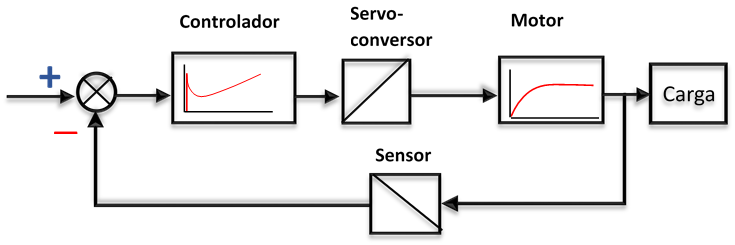
\includegraphics[scale=0.90]{SERVO}
\caption{Control de lazo cerrado de un servomotor}
\end{figure}

\paragraph{Componentes de un servomotor}\leavevmode\newline
Los servos incluyen tres componentes principales: un motor, un variador/amplificador y un mecanismo de retroalimentación.También se incluye típicamente una fuente de alimentación y un servocontrolador capaz de controlar un solo eje o coordinar el movimiento a varios ejes. \\ 

Los servomotores pueden ser del tipo CA o CC, siendo los servomotores de CA los más adecuados para aplicaciones de velocidad constante y los servomotores CC para aplicaciones de velocidad variable. \\ 

La retroalimentación es proporcionada normalmente por un codificador o encoder (ya sea interno o externo). En aplicaciones que requieren un posicionamiento muy preciso, se pueden utilizar dos dispositivos de retroalimentación: Uno en el motor para verificar el rendimiento del motor y otro en la carga para verificar la posición real de la carga. \\ 

Un servo-accionamiento amplifica la señal de un controlador maestro proporcionando suficiente corriente(potencia) al motor para generar velocidad y producir par. En un motor rotativo, la corriente es proporcional al par, por lo que el servomotor controla directamente el par producido por el motor. \\

Del mismo modo, en un motor lineal, la corriente es proporcional a la fuerza, por lo que el accionamiento controla la fuerza producida por el motor. \\ 

El servomocontrolador (también conocido como controlador de movimiento) puede ser considerado como el cerebro del sistema del servomotor. Aquí es donde reside el perfil de movimiento, incluyendo aceleración, velocidad y desaceleración deseadas.\\ 

El controlador envía señales al convertidor, lo que hace que el motor ejecute el movimiento deseado. También tiene la importante tarea de cerrar el bucle en el sistema leyendo la retroalimentación del encoder y modificando la señal del motor (a través del convertidor) para corregir cualquier error en la posición real frente a la deseada, velocidad o par. \\ 

\begin{figure}[htbp]
\hspace*{4.2cm} 
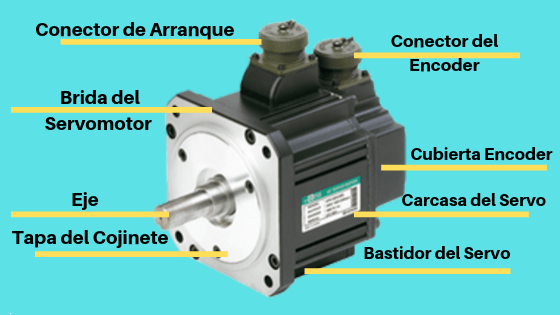
\includegraphics[scale=0.65]{PARTES_SERVO}
\caption{Partes externas del servomotor}
\end{figure}

\paragraph{Ventajas y desventajas de servomotores}\leavevmode\newline
\paragraph*{Ventajas:}\leavevmode\newline
\begin{itemize}
\item Si se coloca una carga pesada en el motor, el servo-controlador aumentará la corriente en la bobina del motor mientras intenta girar el motor. Básicamente, no hay ninguna condición fuera de los pasos. \\
\item El funcionamiento a alta velocidad es posible. \\ 
\end{itemize}
\paragraph*{Deventajas:}\leavevmode\newline
\begin{itemize}
\item Dado que el servomotor trata de girar de acuerdo a los pulsos de mando, pero se queda atrás, no es adecuado para el control de precisión de la rotación.
\item Mayor costo. 
\item Cuando está parado, el rotor del motor continúa moviéndose hacia adelante y hacia atrás con un pulso, por lo que no es adecuado si necesita evitar la vibración. 
\end{itemize}

\paragraph{Aplicaciones}\leavevmode\newline
Los servomotores se utilizan en aplicaciones que requieren variaciones rápidas de velocidad sin sobrecalentar el motor. \\

Algunas de sus aplicaciones son: \\

\begin{itemize}
\item En las industrias se utilizan máquinas herramienta, embalaje, automatización de fábricas, manipulación de materiales, conversión de impresión, líneas de ensamblaje y muchas otras aplicaciones exigentes; robótica, maquinaría CNC o fabricación automatizada. 
\item También se utilizan en aviones radio-controlados para controlar la posición y el movimiento de los ascensores. 
\item Se utilizan en robots debido a su suave encendido y apagado y a su preciso posicionamiento. 
\item También se utilizan en la industria aeroespacial para mantener el fluido hidráulico en sistemas hidráulicos. 
\item Se utilizan en juguetes controlados por radio. 
\item Se utilizan en dispositivos electrónicos tales como DVDs, reproductores de discos o impresoras. 
\item También se utilizan en automóviles para mantener la velocidad de los vehículos. 
\end{itemize}

\begin{figure}[htbp]
\hspace*{4.2cm} 
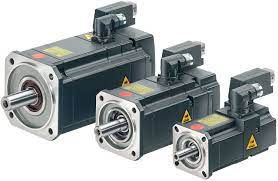
\includegraphics[scale=0.70]{servomotores}
\caption{Servomotores industriales}
\end{figure}
\newpage
\section{ Desarrollo de actividades}
Como en todo inicio de proyecto, se debe de comenzar con la definición de tareas y actividades que el proyecto tendrá para alcanzar el objetivo final. Esta planificación de actividades se debe de definir con una aproximación del tiempo en que se necesita llevar a cabo cada una de las actividades. \\ \\

Siguiendo con esta metodología, a  continuación se presenta el cronograma general de actividades para llevar a cabo el proyecto de residencia. \\ \\
\subsection{Cronograma de Actividades}
\begin{figure}[htbp]
\hspace*{0.8cm} 
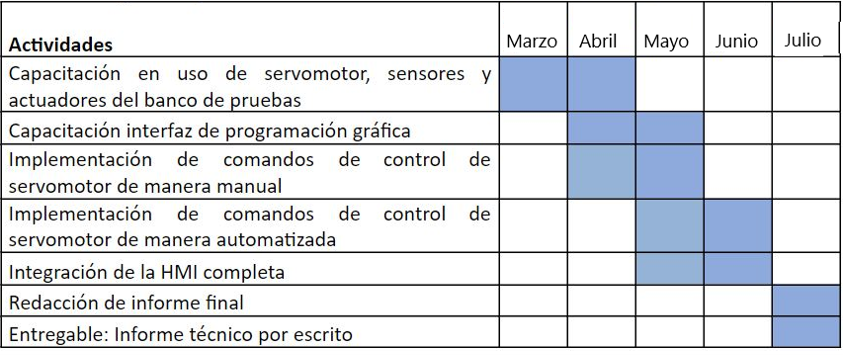
\includegraphics[scale=0.70]{cronograma}
\caption{Cronograma general del proyecto de residencia}
\end{figure}


El anterior cronograma fue el cronograma preliminar presentado al inicio del proyecto, en esencia general son las tareas que se llevaron a cabo a lo largo del desarrollo, algunas tareas se integraron al cronograma, otras tareas se modificaron, pero en relación al tiempo de ejecución de cada una, se siguió de forma correcta. \\
\newpage
\subsection{Definición de proyecto}
El proyecto consiste en desarrollar un control y monitoreo de un banco de pruebas que CIATEQ Zapopan comenzó a desarrollar, pero que se encuentra semi-automatizado. Es por ello que el trabajo de este proyecto de residencia es llevar a cabo la integración de los dispositivos actuales a una sola plataforma de control, y así dar inicio a la automatización del banco de pruebas a través de una aplicación de escritorio o HMI, donde se pueda generar pruebas a la máquina eléctrica desde la aplicación. \\  

El banco de pruebas debe de funcionar en dos modos de operación, uno en modo motor y otro en modo generador. 
\subsubsection{Modo Motor}
Lo que se pretende realizar en el modo motor es utilizar el banco de pruebas como un monitor de comportamiento de un motor externo, conectado al banco de pruebas. \\

El siguiente diagrama a bloques muestra como los dispositivos del banco de pruebas están organizados: \\ 
\begin{figure}[htbp]
\hspace*{0.2cm} 
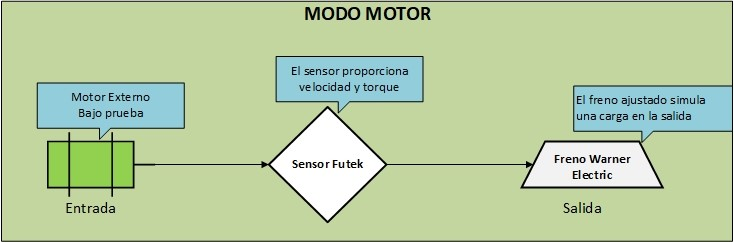
\includegraphics[scale=0.90]{MODO_MOTOR}
\caption{Diagrama a bloques modo motor}
\end{figure}

Como se observa, en el modo motor se coloca un motor en la entrada del sistema (ilustrado en color verde),  este motor es el que se va a poner bajo prueba de funcionamiento.

\vspace{5mm}

El siguiente elemento es el sensor Futek, este sensor nos va a proporcionar información de velocidad y torque que el motor esta ejerciendo. \\

Por último se tiene la salida, el cual para fines de simulación de una carga colocada en el motor, se utiliza  un freno Warner Electric en modalidad de freno ajustado, para simular una carga.\\
\newpage
\subsubsection{Modo Generador}
En el modo generador, el banco de pruebas se utiliza para poner bajo prueba un generador eléctrico que se encuentra en la salida del sistema. \\ 

El siguiente diagrama a bloques muestra como los dispositivos del banco de pruebas están organizados: \\ 

\begin{figure}[htbp]
\hspace*{0.45cm} 
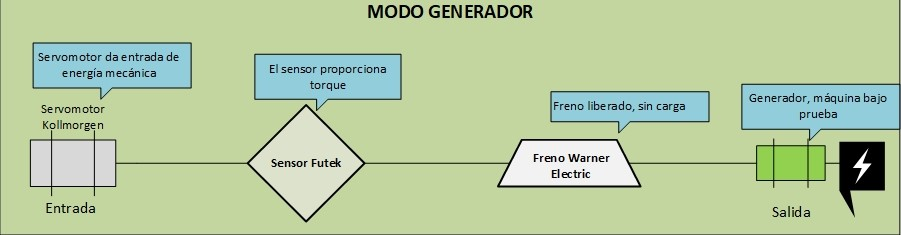
\includegraphics[scale=0.70]{Modo_Generador}
\caption{Diagrama a bloques modo generador}
\end{figure}

Como se puede observar en el diagrama de bloques, en el modo generador se tiene en la entrada del sistema un servomotor Kollmorgen, este servomotor simulará la energía mecánica que entra al eje de distribución, el segundo elemento encontrado es el sensor Futek, que únicamente nos proporciona la información del torque mecánico. \\ 

El tercer elemento encontrado en el sistema es el freno Warner Electric, estre freno debe de estar en modalidad libre para no añadir una carga extra al sistema. \\ 

Por último, se tiene la salida, donde se tiene el generador eléctrico bajo prueba, generando la diferencia de potencial en sus terminales. \\

Con base a lo anterior, se tiene una mejor idea de como el banco de pruebas debe de trabajar, y son escenarios de trabajo que se deben de tener en cuenta para el desarrollo del control e interfaz gráfica. \\ 

\subsubsection{Primeras ideas}
Como primeras ideas, se tienen por lo tanto que el \textbf{sistema de control} debe de ser capaz de soportar cambios de modalidad, por lo cual se debe de tener en cuenta que dentro del código del programa de control deben de existir dos bloques, uno para el control del modo motor, y otro para el modo generador. \\ 

Dentro de cada bloque, se encuentran los recursos en código de control para los dispositivos del banco de pruebas. \\
\newpage
Por otro lado, para el desarrollo de la \textbf{interfaz gráfica de usuario}, esta debe de permitir cambios de modos de operación, entre modo motor y modo generador, por lo cual se debe de tener una interfaz gráfica con por lo menos 3 ventanas principales: \\

\begin{itemize}
\item Ventana principal
\item Ventana modo motor. 
\item Ventana modo generador.
\end{itemize}

Se debe de definir que información de interés se deben de mostrar en las ventanas, por lo tanto:  \\
\paragraph*{Ventana principal:} En esta ventana el usuario tendrá que hacer comunicación con el controlador, saber que el controlador esta en comunicación con la GUI, una vez comunicado, se podrá elegir del menú de opciones el modo en el que se desea trabajar, sea modo motor o modo generador. 
\paragraph*{Ventana modo motor:} En esta ventana el usuario podrá observar los datos del sensor futek (velocidad y torque) así como también controlar la liberación y activación del freno ajustado. 
\paragraph*{Ventana modo generador:} Esta ventana es la ventana más elaborada de la interfaz gráfica, ya que el usuario dentro de esta ventana podrá observar el monitoreo de señales y el ajuste de movimiento. \\[0.8cm]

Con esta sección se aborda la definición del proyecto, que es parte fundamental para cualquier desarrollo de diseños en ingeniería, al tener definido el proyecto, se tiene un panorama más claro de como es que se va a desarrollar el proyecto, de igual manera surgen preguntas tales como: \\

\begin{itemize}
\item ¿Qué dispositivos son los que se tienen en el banco de pruebas?
\item ¿Cómo se comunican?
\item ¿Cómo controlo y recibo información?
\item ¿Qué controlador utilizar para la aplicación?
\item ¿En que plataforma desarollar la GUI? 
\end{itemize}

Las anteriores preguntas es el siguiente paso del desarrollo, serán contestadas en las siguientes secciones. \\
\newpage
\subsection{Reconocimiento de dispositivos}
El banco de pruebas a máquinas eléctricas que CIATEQ Zapopan comenzó a desarrollar consiste de los siguientes elementos: \\
\begin{itemize}
\item Kollmorgen Servomotor AKM65K-ACCNR-00
\item Kollmorgen Servodrive AKD-P01206-NBEC-0000
\item Sensor de torque y velocidad FUTEK TRS605
\item Freno Warner Electric CBC-550-90
\end{itemize}

Lo anteriores elementos son los que se encuentran ya en el banco de pruebas pero no hay ninguna plataforma general en el cual estos elementos interactuen en conjunto para poder realizar pruebas a máquinas eléctricas.\\

Para poder continuar con el desarrollo del proyecto, primeramente se debe de realizar una caracterización de que plataforma de control es la más adecuada para la interacción con los anteriores elementos, tomando en cuenta la comunicación para poder leer y escribir información. \\ 

\subsubsection{Kollmorgen Servodrive y Servomotor}
El servomotor Kollmorgen AKM65K-ACCNR-00 necesita trabajar en conjunto con el servodrive Kollmorgen AKD-P01206-NBEC-0000, por lo tanto, el servomotor trabajará bajo ordenes del servodrive. \\

Con lo anteriormente dicho, se observa que nuestro objetivo es el estudiar el servodrive, y no el servomotor, puesto que dominando y controlando al servodrive, podremos hacer que el servomotor trabaje bajo nuestras ordenes, teniendo al servodrive como interprete intermediario en la comunicación. \\ 

\begin{figure}[htbp]
\hspace*{2.5cm} 
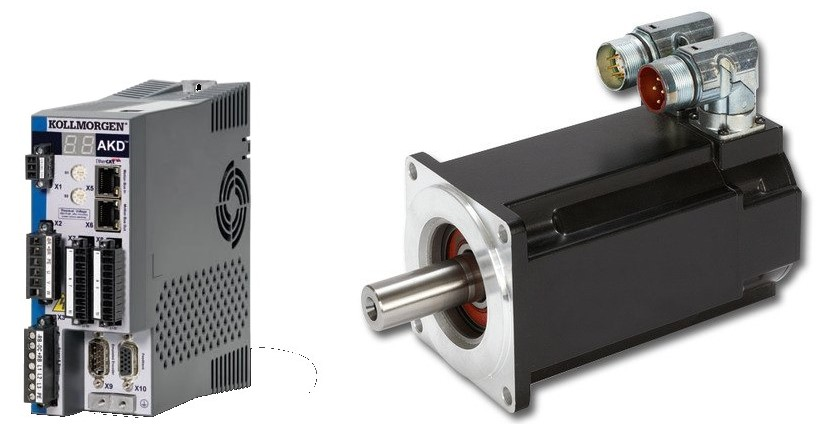
\includegraphics[scale=0.55]{kollmorge_devices}
\caption{Dispositivos Kollmorgen en banco de pruebas}
\end{figure}
\newpage
Nuestro objetivo principal será el conocer el servodrive, por lo tanto se realizó un estudio del manual de usuario propio del servodrive Kollmorgen AKD-P01206-NBEC-0000 para controlar dispositivo servomotor Kollmorgen AKM65K-ACCNR-00. \\ 

En primer instancia la manera de poder realizar movimientos con el servomotor, obtener datos propios del servodrive y servomotor es dando uso al software que el fabricante proporciona, este sofware es llamado "Kollmorgen WorkBench" \\ 

\begin{figure}[htbp]
\hspace*{2.5cm} 
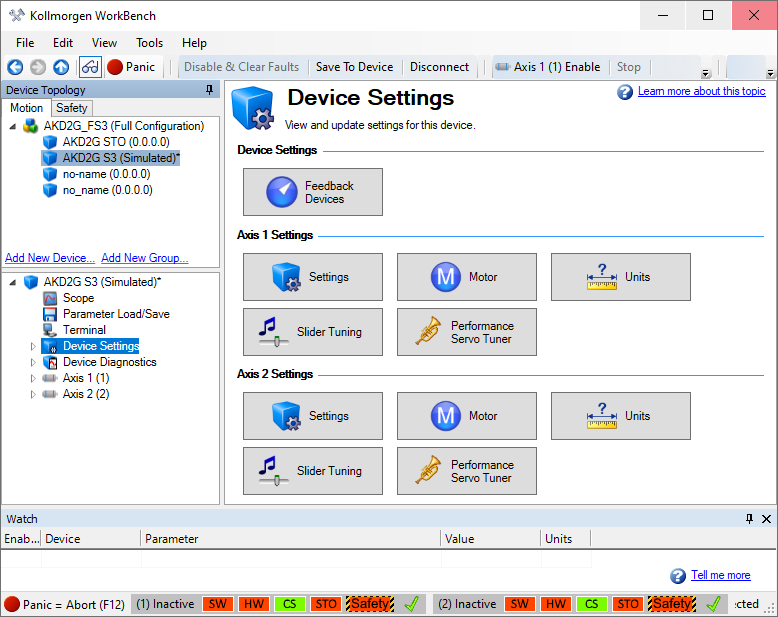
\includegraphics[scale=0.55]{WorkBench_0}
\caption{Software  Kollmorgen WorkBench}
\end{figure}

Con ayuda de este software, se pueden realizar movimientos del servomotor con una configuración establecida por el propio usuario.\\

Este software tiene muchas funciones, muchos datos recopilados, incluso te muestra gráficas de comportamiento y también se pueden crear recetarios de perfiles de movimiento para poder cargarlos directamente. \\ 

Este software fue la parte inicial para conocer y aprender como se generan movimientos específicos que el usuario desea realizar. \\ 

Para poder dar uso a este software y controlar los dispositivos Kollmorgen solamente se debe de dar uso a una comunicación ethernet de computadora a servodrive, el programa automáticamente reconoce el dispositivo a través de su IP definida y se abre el software para dar inicio a la configuración de perfiles de movimiento. \\ 

\newpage
Una vez que se dominó como configurar diferentes movimientos, se comenzó con la investigación sobre que tipo de comunicación (bus de campo) utilizar para el proyecto. \\ 

El servodrive se puede comunicar a través de algún  bus de campo tales como: \\
\begin{itemize}
\item EtherCat 
\item Modbus 
\item Ethernet TCP /IP
\end{itemize}

A partir de este punto, se debe de tener en mente que tipo de comunicación debe de soportar el sistema de control para que se pueda comunicar con el servodrive. \\ 

Pero este tema se verá más adelante, por el momento, este fue el primer paso para cononocer los dispositivos Kollmorgen que el banco de pruebas tiene y poder ver en funcionamiento el servomotor realizando los movimientos que se establecen previamente en el software Kollmorgen WorkBench. \\ 

\subsubsection{Sensor de velocidad y torque Futek } 
El banco de pruebas tiene un sensor de velocidad y torque Futek TRS605. Este sensor no es tan complejo como los dispositivos Kollmorgen que se vieron en el apartado anterior, ya que este sensor entrega señales de salida para el propio controlador. \\

Este sensor nos entrega el dato del velocidad y torque. \\ 

\begin{figure}[htbp]
\hspace*{5.5cm} 
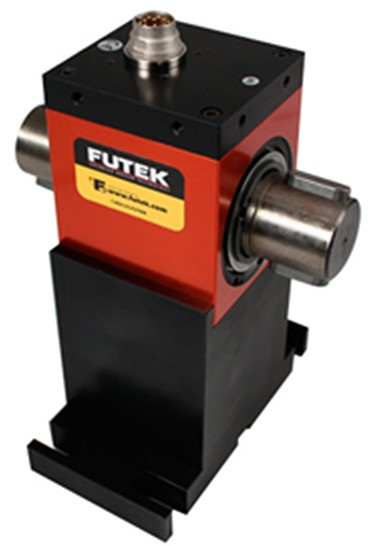
\includegraphics[scale=0.55]{TRS605}
\caption{Sensor FUTEK TRS605}
\end{figure}
\newpage
\paragraph{Dato de velocidad}\leavevmode\newline

Para obtener el dato de velocidad, se debe de tomar en cuenta las terminales que nos entregan ese dato, dando uso a la hoja técnica del propio sensor: \\

\begin{figure}[htbp]
\hspace*{5.2cm} 
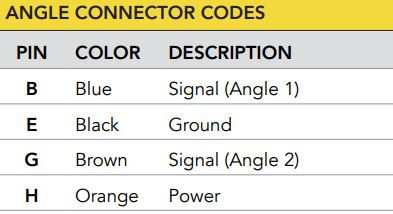
\includegraphics[scale=0.58]{dato_velocidad_pin}
\caption{Terminales involucradas para dato velocidad}
\end{figure}

Para obtener el dato de velocidad, es necesario conectar del siguiente modo las anteriores terminales: 
\begin{itemize}
\item \textbf{Blue:} Esta terminal es el ángulo 1, debe de ser leída por el controlador. 
\item \textbf{Black:} Esta terminal es ground o por su traducción tierra, conectarla a tierra  del sistema. 
\item \textbf{Brown:} Esta terminal es el ángulo 2, debe de ser leída por el controlador. 
\item \textbf{Orange:} Esta terminal es power, debe de ser conectada a +5V 
\end{itemize}

Las terminales de ángulo son las que nos entregan los valores necesarios para determinar la velocidad, esta señal debe de ser leída a través de un controlador que tenga interrupciones, puesto que de esta manera es leída esta señal.\\

A través de las interrupciones, se establece una temporización entre el ángulo 1 y ángulo 2  para medir su desfase entre una y otra y así se determina la velocidad de giro y la dirección en la que gira el eje. \\ 

Como se puede deducir entonces, el ángulo 1 y el ángulo 2 son señales cuadráticas, las cuales son pulsos cuadrados que se modifican de acuerdo a la velocidad y giro del eje, como se puede apreciar en la siguiente imagen:  

\begin{figure}[htbp]
\hspace*{4.5cm} 
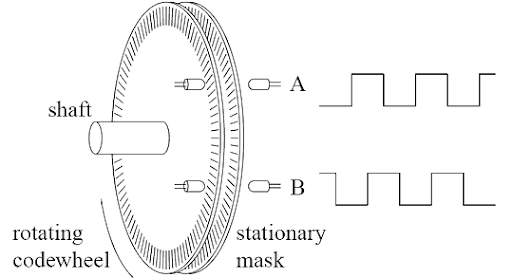
\includegraphics[scale=0.40]{signals_encoder}
\caption{Señales cuadráticas de encoder}
\end{figure}
\newpage
\paragraph{Dato de torque}\leavevmode\newline

Para obtener el dato de torque, es necesario conocer las siguientes terminales: \\ 
\begin{figure}[htbp]
\hspace*{5.2cm} 
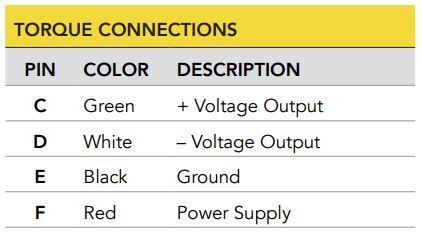
\includegraphics[scale=0.58]{dato_torque_pin}
\caption{Terminales involucradas para dato torque}
\end{figure}

Para obtener el dato del torque, es necesario conectar del siguiente modo las anteriores terminales: 
\begin{itemize}
\item \textbf{Green:} Esta terminal es la salida de voltaje positivo, debe de ser leída por el controlador. 
\item \textbf{White:} Esta terminal es la salida de voltaje negativo, debe de ser leída por el controlador. 
\item \textbf{Black:} Esta terminal es ground o por su traducción tierra, conectarla a tierra  del sistema.
\item \textbf{Red:} Esta terminal es Power, debe de ser conectada a +12V 
\end{itemize}

Para poder reconocer el dato del torque, se deben de tratar las señales de voltaje positivo y negativo como dos señales analógicas en el sistema, con la observación de que, son señales diferenciales por lo cual se deben de acondicionar sea en el propio sistema de control, o usando algún hardware externo al sistema, para dejar una señal acondicionada para ser leída por el controlador. \\

\subsubsection{Freno industrial Warner Electric } 
El siguiente dispositivo a reconocer es el freno industrial Warner Electric CBC-550-90. Este dispositivo es un freno industrial el cual cuenta con su controlador propio, pero a diferencia del controlador del servomotor, este  puede ser accionado por un controlador master a través de señales digitales. \\ 

El propósito de este dispositivo en el banco de pruebas es para generar alguna resistencia o carga en el sistema cuando el banco de pruebas se encuentra operando en el modo motor, y que cuando el banco de pruebas se encuentre trabajando en modo generador, se encuentre libre de carga en el sistema, osea sin freno. \\ 
\newpage
Lo interesante de este dispositivo, es que tiene 3 modalidades de operación: 
\begin{itemize}
\item Freno total
\item Freno Ajustado
\item Freno Libre
\end{itemize}
 
 En \textbf{Freno total} como su nombre lo indica, esta totalmente amarrado al sistema, no puede generar ningún movimiento el eje del freno, ya que el freno mecánico ha sido accionado. Este modo para el proyecto no es necesario implementarlo, puesto que significa un peligro, ya que si se llegará  accionar accidentalmente este tipo de modo  cuando se encuentra el banco de pruebas ejecutando una prueba,  puede correr un riesgo significativo para el banco, por lo cual se debe de implementar una solución para prevenir este modo de operación de freno. \\ 
 
 En \textbf{Freno ajustado}, este modo de operación permite accionar un tipo de freno ajustado, el cual este modo de operación será utilizado como una simulación de una carga extra en el sistema cuando se encuentra trabajando en modo motor. El ajuste se realiza a través de un potenciómetro embebido que se tiene en la tarjeta de control/potencia del freno, y el ajuste se debe de realizar de manera manual. \\ 
 
En \textbf{Freno libre}, en este modo el freno se encuentra libre, no debe de añadir carga extra al sistema, por lo cual este modo de operación de freno será utilizada cuando se encuentre el banco de pruebas en modo generador. \\ 
  
De manera física, los dispositivos son los siguientes: \\
\begin{figure}[htbp]
\hspace*{2.2cm} 
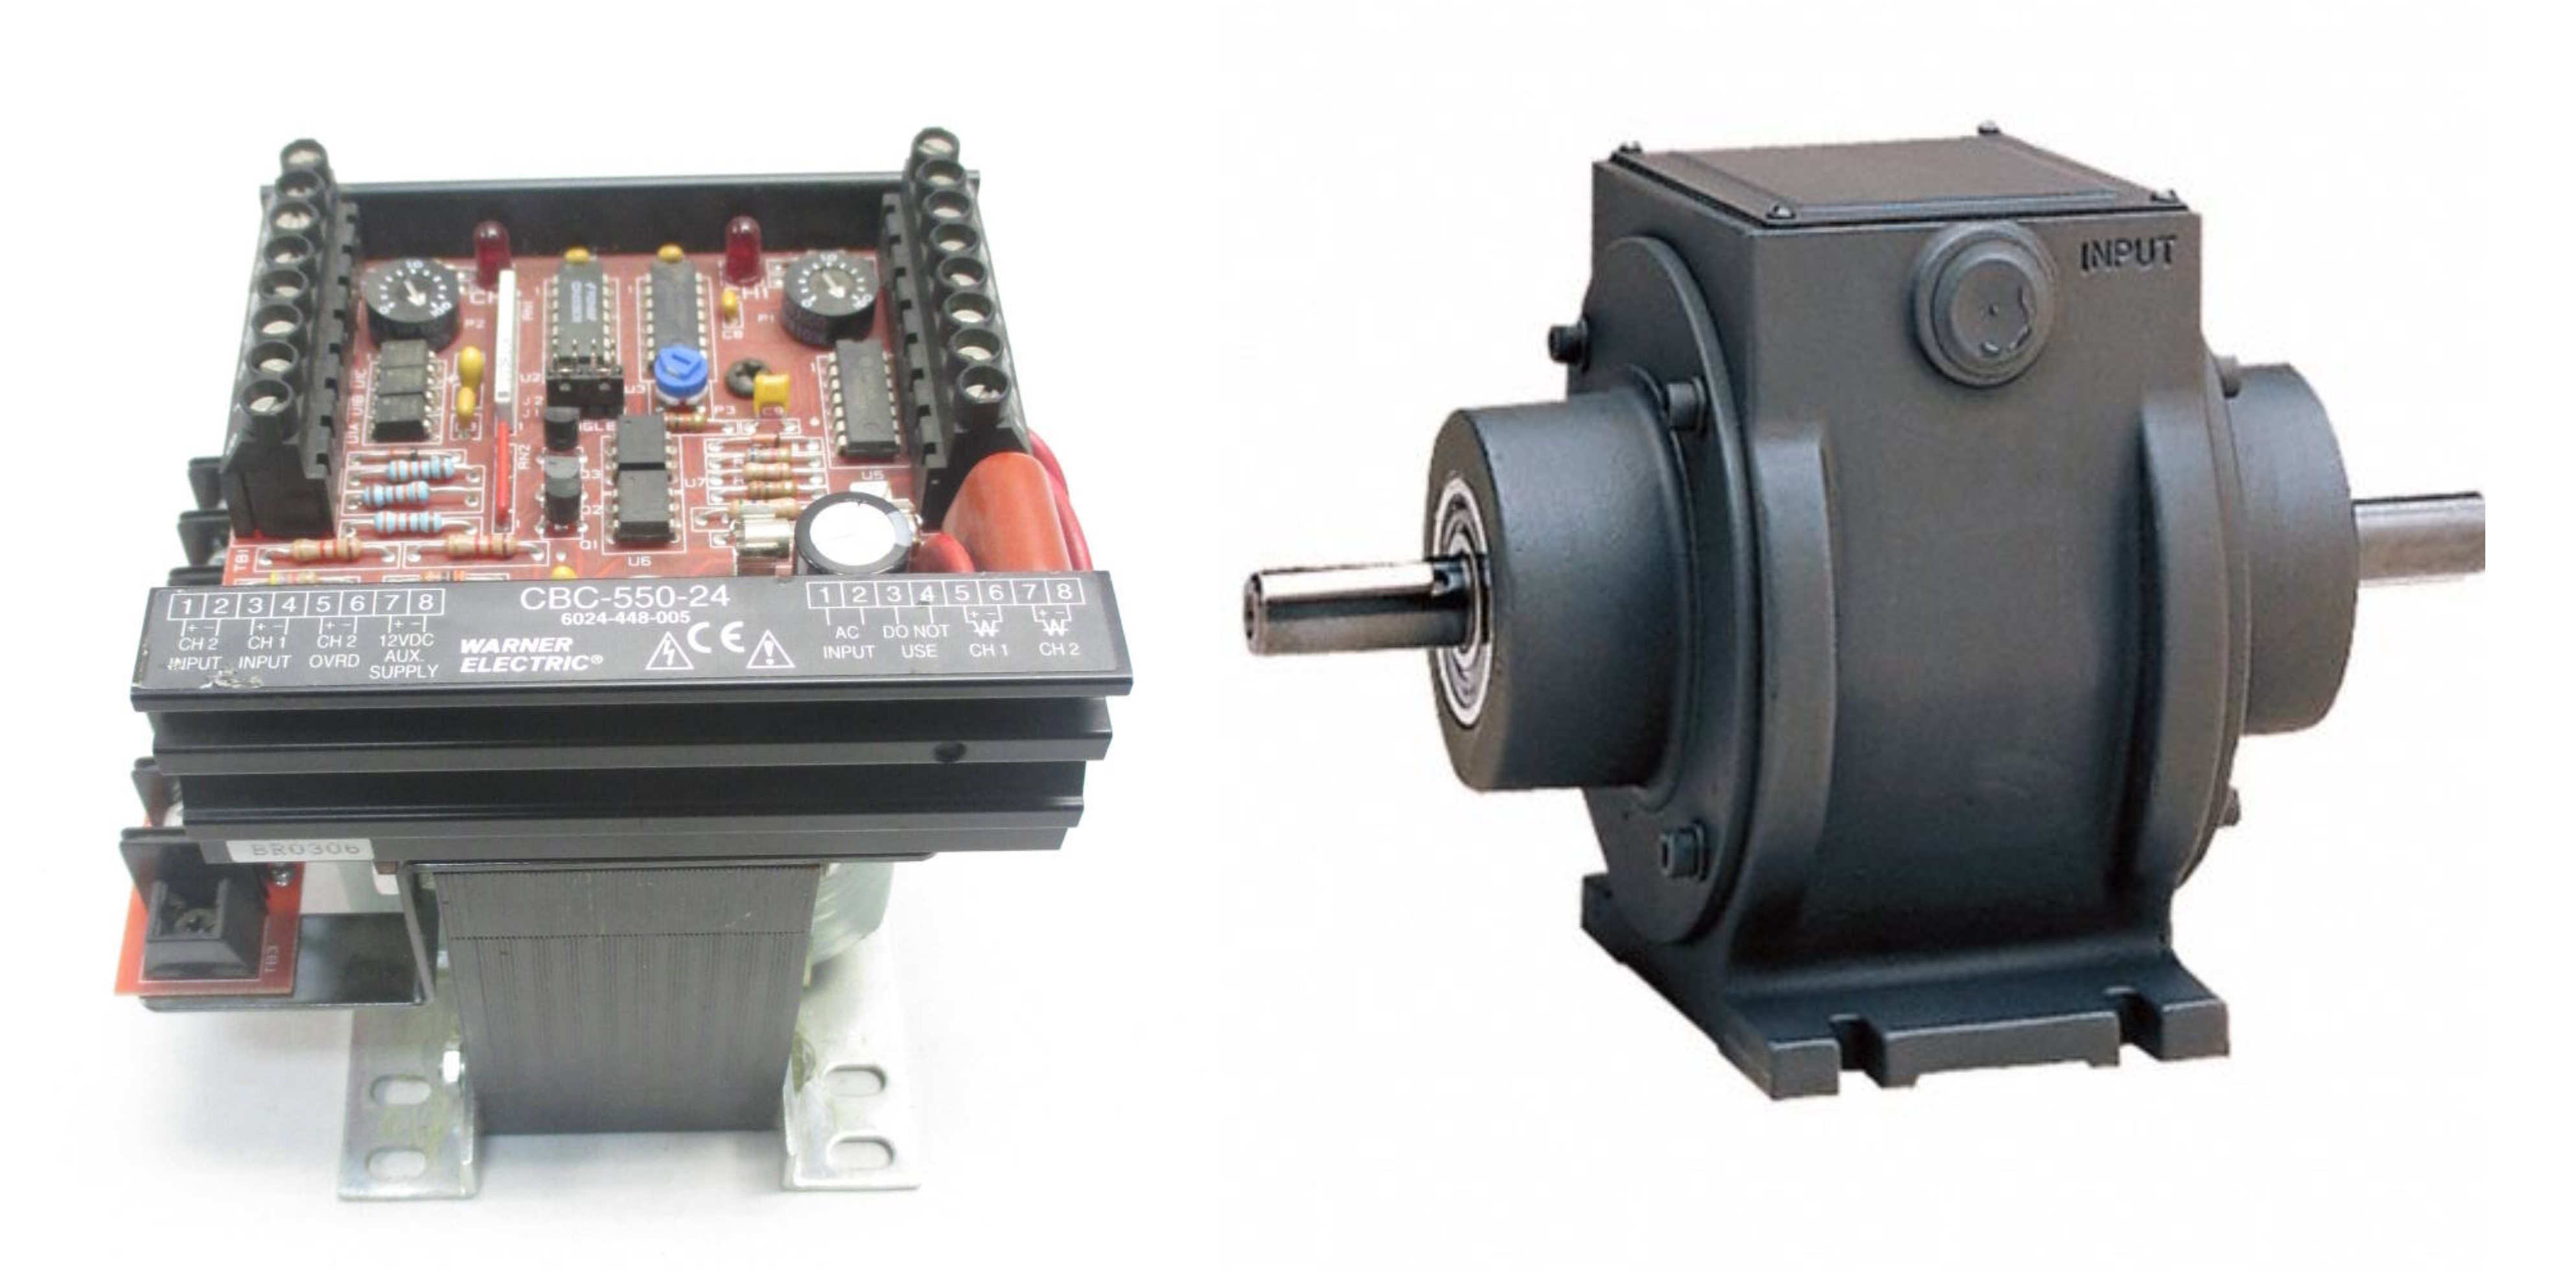
\includegraphics[scale=0.13]{warner_devices}
\caption{Controlador y freno industrial Warner Electric}
\end{figure}
\newpage
Para poder controlar el freno industrial se debe de seguir la siguiente tabla: \\
 
\begin{figure}[htbp]
\hspace*{5.2cm} 
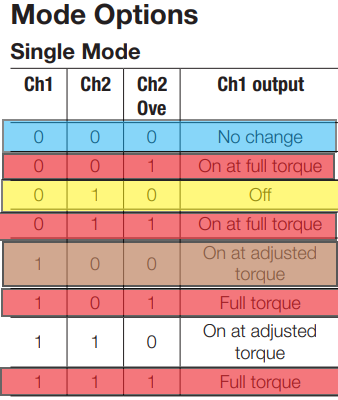
\includegraphics[scale=0.69]{modos_freno}
\caption{Tabla lógica de control Freno Warner Electric}
\end{figure}

La anterior tabla lógica se encuentra marcada con colores de los modos de operación que son de interés en el proyecto, el cual a continuación se describen cada uno: 

\begin{itemize}
\item \textbf{Azul: } El color azul será utilizado como "No change", se mantendrá en un modo comportándose como latch. 
\item \textbf{Amarillo: } En el color amarillo se encuentra el modo generador, en otras palabras el freno se encuentra libre. 
\item \textbf{Café: } En el color café se encuentra el modo motor, el freno se encuentra en un torque ajustado. 
\item \textbf{Rojo: } En el color rojo se encuentra el estado donde el freno mecánico se encuentra presente, estos estados se deben de evitar. 
\end{itemize}

Al analizar la tabla anterior se puede observar que en los estados lógicos que significan un peligro para el banco de pruebas (los marcados en rojo) hay una entrada denominada \textsc{CH2 OVE} que se encuentra en '1' lógico siempre, y que en los tres estados lógicos que vamos a utilizar para el proyecto, esa entrada se mantiene en '0' lógico, por lo cual una forma garantizada de que nunca vamos a entrar en el estado lógico de color rojo es aterrizando a '0' lógico la entrada \textsc{Ch2 ove} y así vamos a evitar ese estado lógico no deseado en el sistema. \\ 

Por último, observamos entonces que para poder controlar el freno adecuadamente para el sistema, será necesario dar uso a las entradas \textsc{Ch1} y \textsc{Ch2} siguiendo los estados lógicos marcados en azul, amarillo y café.  

\newpage
Como se observó en esta sección, se dio inicio al reconocimiento de los dispositivos encontrados en el banco de pruebas y ya tenemos un bosquejo de que tipo de controlador se debe de utilizar.\\

El sistema de control que se debe de utilizar entonces, debe de soportar lo siguiente: 
\begin{itemize}
\item Comunicación industrial para servodrive (EtherCat,Modbus,Ethernet TCP IP).
\item Pines de entrada con interrupción (x2) para Sensor Futek.
\item Pines de entrada analógica diferencial (x2) para Sensor Futek.
\item Pines de salida digital (x2) para freno industrial.
\end{itemize} 

Por lo tanto, este dato es lo mínimo que se requiere para el sistema de control, que será analizado en la siguiente sección. \\ 

\subsection{Propuestas de controlador}
Para la elección del controlador del proyecto, se tienen los siguientes dispositivos posibles a utilizar: \\ 

\begin{itemize}
\item \textit{Raspberry Pi 3B}
\item \textit{Arduino UNO}
\end{itemize}

\subsubsection{Raspberry Pi}
La raspberry Pi como definición es una mini computadora embebida con un procesador Broadcom BCM2837B0.\\

Este sistema embebido es muy utilizado en proyectos orientados a la mecatrónica e informática, lo que hace interesante una raspberry es que cuenta con un procesador, el cual a este se le carga una imagen de algún sistema operativo, sea Windows, o alguna distribuición de Linux. Logrando así tener un recurso adicional para proyectos orientados a la mecatrónica. \\ 

Teniendo el recurso de tener un sistema operativo en la propia tarjeta embebida, se pueden desarrollar proyectos mecatrónicos más robustos que cuando se usa un microcontrolador, puesto que con el sistema operativo o mejor dicho con ayuda del procesador, se pueden crear proyectos donde se den uso a los pines GPIO de la raspberry, se tome lectura de sus entradas y salidas, y que además los datos sea almacenados en una nube directamente. \\ 

Teniendo un sistema operativo en el proyecto, se abren muchas posibilidades de continuar con el desarrollo, incluso involucrando tecnologías IoT. \\ 

\newpage

Para el proyecto de residencia se da como propuesta usar Raspberry Pi como controlador del proyecto, ya que la Raspberry tiene la capacidad de soportar comunicación EtherCat y Modbus, ya que la tarjeta tiene un slot Ethernet embebida.\\ 

Se pretendía usar una plataforma llamada Codesys el cual es una plataforma donde la Raspberry la podemos controlar como si fuera un PLC. \\ 

Al utilizar Codesys, se podría cargar la configuración propia de una comunicación Modbus o EtherCat que el servodrive Kollmorgen soporta y así poder comunicarnos con la tarjeta de control.\\ 

Posterior a ello, la configuración de los espacios de memoria (registros de configuración) Kollmorgen pudieran haber sido de manera más rápida, ya que se encontró el archivo de configuración GSD del servodrive para cargarlo a Codesys.\\

Además otra ventaja de usar Raspberry sería su capacidad de correr multitareas o como se le conoce en informática "multithreading" para tener la ventaja de correr dos o tres tareas al mismo tiempo sin afectar el proceso de ejecución del programa. \\ 

Pero una desventaja que se observó con esta propuesta es que para utilizar algunas funciones requeridas para el proyecto por parte de Codesys, entraba en juego una licencia de pago para poder usar esas características, por lo cual la propuesta quedó por un lado. \\

Pero sin duda alguna, trabajar con Raspberry Pi bajo la plataforma de Codesys se pudieran desarrollar proyectos muy interesantes. \\

\begin{figure}[htbp]
\hspace*{4.8cm} 
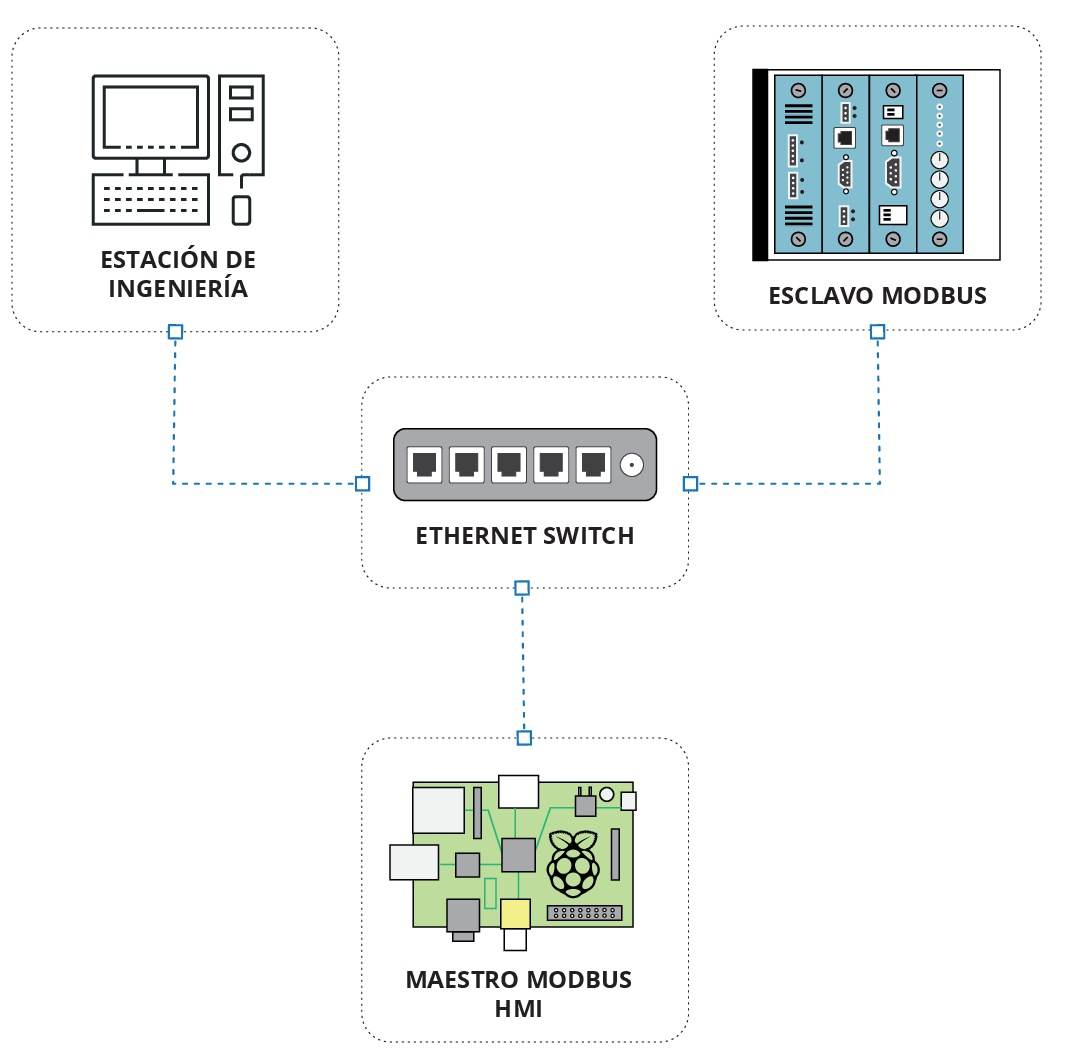
\includegraphics[scale=0.49]{bloq_diagram}
\caption{Red de comunicación Raspberry Pi}
\end{figure}
  
\subsubsection{Arduino}
El arduino Uno como se vio en la parte de teoría, es un sistema embebido el cual cuenta con un microcontrolador Atmega328p AVR de 8 bits, el arduino funciona de manera excelente para proyectos de pequeña escala el cual el fabricante indica que es una tarjeta de enseñanza para la  inicialización al mundo de la programación de microcontroladores. \\ 

En la mayoría de universidades, el arduino forma parte de la enseñanza en asignaturas como "programación de microcontroladores", "programación de sistemas embebidos", entre otros. \\

Para el proyecto de residencia se toma en cuenta la capacidad del arduino uno para utilizarlo como controlador general del banco de pruebas a máquinas eléctricas, únicamente se debe de contemplar que cumpla con los requisitos mínimos que los dispositivos del banco de pruebas requieren. \\

Por lo tanto se comenzó con la investigación de como realizar una comunicación EtherCat o Modbus para poder enlazar la comunicación de Arduino a Servodrive bajo alguno de estos dos protocolos de comunicación. \\ 

Se comenzó con la investigación de EtherCat, si era posible realizar ese tipo de protocolo de comunicación en arduino Uno, el cual la información que se encontró no estaba del todo clara de como realizar una comunicación bajo este protocolo, por lo cual se decide por investigar con más profundidad la comunicación Modbus TCP/IP en arduino. \\ 

En la etapa de investigación se encontró un curso que ayudó bastante para observar que el arduino puede soportar comunicación Modbus TCP/IP, este curso se encuentra en la página Udemy.com, el nombre del curso es \textit{" How to program an Arduino as a Modbus TCP/IP Client and Server"} curso realizado por el instructor Emile Ackbarali. \\

Con el anterior curso, logré realizar pruebas de comunicación Modbus TCP/IP entre Arduino UNO y PC, usando un simulador de interpréte Modbus, pude observar la comunicación y la manera de interactuar escribiendo y leyendo registros de modbus a través de arduino, siendo este un cliente en la comunicación y la computadora un servidor. \\

Con base a la experiencia anterior, se encuentra una manera eficiente para establecer la comunicación al servodrive Kollmorgen, únicamente se tendría que revisar los registros involucrados para la configuración correcta del servodrive y hacer pruebas de lectura/escritura, esta etapa se verá más adelante, por el momento se llega a una solución para establecer la comunicación Modbus TCP/IP desde el arduino funcionado como cliente. \\

\newpage

Cabe mencionar que el arduino no tiene slot ethernet, por lo tanto para realizar esta comunicación se dió uso al \textit{ethernet shield  for arduino} para darle la capacidad al arduino.\\ 

\begin{figure}[htbp]
\hspace*{4.2cm} 
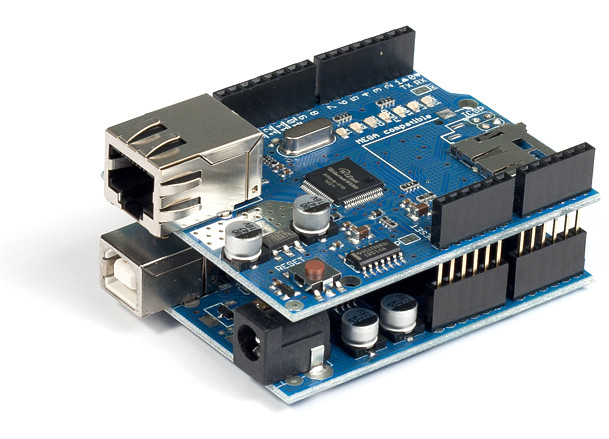
\includegraphics[scale=0.39]{Arduino_ethernet}
\caption{Arduino Uno con Arduino Ethernet Shield}
\end{figure}

Además del shield, se dieron uso a las siguientes librerias para realizar la comunicación Modbus, las cuales fueron:\\

\begin{itemize}
\item \textit{ModbusTCP library for the Arduino} 
\item \textit{Ethernet library}
\end{itemize}

Las anteriores librerías son de uso libre para proyectos. \\ 

Una vez concluido de que el arduino puede mantener una comunicación modbus, se comienza a revisar los demás requisitos para los otros dipositivos del banco de pruebas. \\

Para poder controlar el freno industrial Warner Electric, se necesitan salidas digitales del controlador, cosa que el arduino tiene. \\

Para el sensor Futek TRS605, para leer el dato de velocidad se necesita pines de interrupción, cosa que el propio microcontrolador del arduino soporta. \\

Por el lado del dato del torque, es una señal analógica por lo cual el Arduino tiene pines dedicados para señales analógicas. \\

Al final es más que evidente que el arduino ha cumplido con los requisitos para ser el controlador del proyecto de residencia y poder controlar y leer los dispositivos del banco de pruebas. \\ 


\newpage
Por último, se revisan las capacidades de memoria de las diferentes versiones de tarjetas arduino: 

 \begin{figure}[htbp]
\hspace*{2.1cm} 
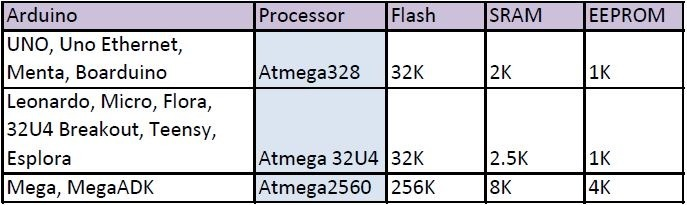
\includegraphics[scale=0.89]{memoria_arduino}
\caption{Comparativa de capacidad de memoria arduino}
\end{figure}

Con base a la anterior comparativa, se observa una significante limitación en la memoria del arduino Uno, tanto en la memoria Flash como en la memoria RAM. \\

Como recordatorio, la memoria Flash es donde se almacena el programa (código) del control, y la memoria RAM es la memoria donde se almacenan datos/variables al ejecutar el programa de control. \\ 

Con la limitada capacidad de memoria del Arduino Uno, se opta por elegir el Arduino Mega como el controlador general del proyecto, dando así la oportunidad de que el microcontrolador Atmega2560 sea el encargado de llevar el control del proceso.\\ 

 \begin{figure}[htbp]
\hspace*{3.8cm} 
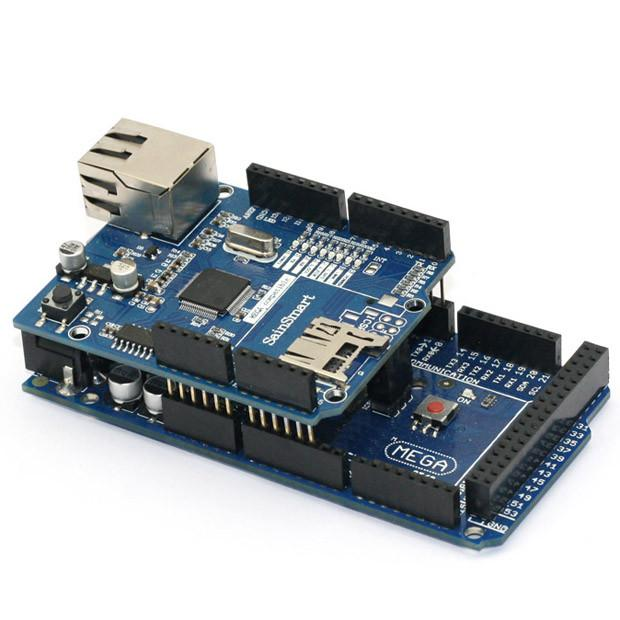
\includegraphics[scale=2.13]{arduino_mega_ethernet}
\caption{Arduino Mega junto con Ethernet shield for arduino}
\end{figure}

\newpage

Al revisar la documentación técnica del encoder Futek TRS605 se observa que para la obtención del dato del torque nos la proporciona en una señal analógica diferencial, esto quiere decir que nos proporciona dos señales analógicas donde una tiene un voltaje positivo y otra tiene un voltaje negativo. \\ 

Esto representa un problema para el microcontrolador de Arduino Mega, en este caso el Atmega2560 ya que sus pines analógicos que tiene son referenciados a tierra, por lo tanto debe de ser un voltaje positivo, y no un voltaje negativo.\\

\begin{figure}[htbp]
\hspace*{3.8cm} 
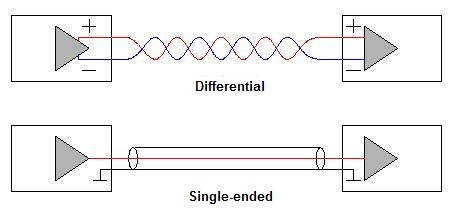
\includegraphics[scale=0.68]{signals_}
\caption{Señal diferencial y señal single ended}
\end{figure}

Por lo tanto se comienza con la investigación de como acondicionar la señal del sensor Futek para ser leída por el microcontrolador, se llega a la solución de dar uso al ADC ADS1115 ya que este ADC cuenta con entradas diferenciales, que pueden leer dichos voltajes del sensor y acondicionarla internamente, una vez que se acondicione la señal, este dato de señal puede ser leído a través de la comunicación I2C, haciendo la comunicación Arduino - ADS1115. \\

\begin{figure}[htbp]
\hspace*{6.1cm} 
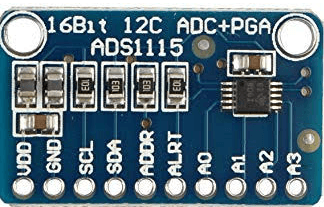
\includegraphics[scale=0.48]{ADS1115}
\caption{ADC ADS1115}
\end{figure}

 


\newpage
\subsection{Propuesta para GUI}
Para el desarrollo de la interfaz gráfica de usuario (GUI) al inicio de la definición del proyecto se estaba contemplando lo siguiente: \\ 

\begin{itemize}
\item \textit{MyOpenLab}
\item \textit{Visual Studio .Net with CSharp}
\end{itemize}

MyOpenLab fue la primer propuesta para la GUI, ya que esta plataforma es libre y es muy utilizada en el campo de la enseñanza de interfaces gráficas. \\

MyOpenLab según la documentación es una herramienta para la programación visual, se usan bloques gráficos para ir desarrollando una aplicación gráfica para el proyecto, algo parecido a MyOpenLab sería Labview, recordando que este último es de pago y esta orientado al desarrollo de VI (Virtual instrument).\\ 

El backend de esta plataforma se encuentra desarrollado en Java. \\ 

Personalmente se comenzó con la investigación de que tan viable sería dar uso a esta plataforma para la GUI del proyecto de residencia, el cual se encontró con algunas fallas a la hora de ejecutar pruebas sencillas con la comunicación arduino, y que además la comunidad de apoyo por parte de otros desarrolladores no se encontraba activa para las fechas del desarrollo del proyecto, por lo cual fueron puntos a tomar en cuenta. También se observó de que si existiera algún problema con algún bloque de función, se debería de depurar directamente en la parte del desarrollo Java para poder resolver el conflicto. \\ 

MyOpenLab puede ser una excelente herramienta para la inicialización del aprendizaje de programación gráfica, para poder crear prácticas o algunos proyectos de pequeña escala, pero para proyectos más grandes sería prudente contemplar otra plataforma con mayor apoyo de la comunidad de desarrolladores, así como también que sea más estable y robusta en sus bloques de funciones. 

 \begin{figure}[htbp]
\hspace*{4.2cm} 
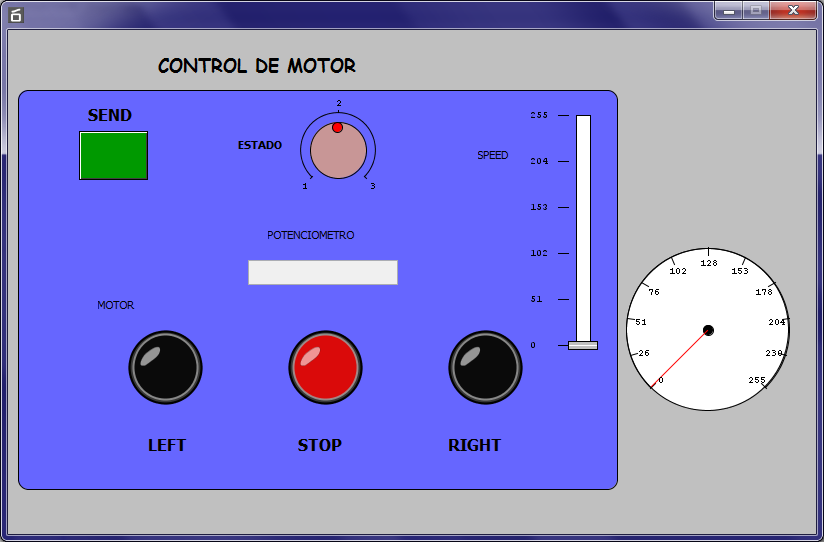
\includegraphics[scale=0.30]{my_openlab}
\caption{Aplicación bajo entorno MyOpenLab}
\end{figure}
\newpage

Es por ello que se empezó a investigar otra propuesta para la GUI, en este caso se encontró la plataforma Microsoft Visual Studio, para dar uso al framework Windows .Net y el lenguaje Csharp para la creación de la GUI. \\ 

 \begin{figure}[htbp]
\hspace*{5.2cm} 

\includegraphics[scale=0.45]{logo_csharp}
\caption{Logo Csharp y Microsoft NET}
\end{figure}

Con una experiencia previa que tuve con Visual Basic en un lugar donde trabajaba, donde logré desarrollar una aplicación de escritorio para la manipulación de un libro de excel para el control de inventarios y generación de listas de materiales, a través de \textit{Visual Basic for Applications Excel }, por lo tanto, cuando observé como se desarrolla una aplicación de escritorio a través de Csharp y el framework Windows .Net de inmediato recordé el desarrollo de aquella aplicación y lo fácil e interactiva que es desarrollar una aplicación a través de código puro. \\

Solo que esta vez, sería utilizando una plataforma nueva para mi carrera de estudiante, sería utilizar Visual Studio community, la tecnología  framework Windows .Net y el lenguaje de desarrollo C sharp, el cual agrega un pequeño desafío en el desarrollo de la GUI, pero que es alcanzable. \\ 

Se dio como propuesta realizar la GUI con las herramientas anteriormente mencionadas y fue aceptada. \\ 

La utilidad de usar framework .net es tener la capacidad de desarrollar aplicaciones de escritorio nativas para el sistema operativo Windows, el cual esta tecnología proporciona al desarrollador herramientas propias para la creación de aplicaciones de escritorio Windows. \\ 

Esta tecnología no únicamente se utiliza para el desarrollo de aplicaciones de escritorio, si no que también tiene utilidad en el desarrollo de aplicaciones móviles, aplicaciones web, desarrollo de interfaces, etc. \\

Por lo tanto, utilizar framework .net junto con C sharp desgloza muchas posibilidades, pero sus capacidades de estas herramientas son explotadas en carreras de ingeniería de desarrollo software o informática. \\

Como se puede deducir, al crear la GUI del proyecto con estas herramientas, se mezclan dos áreas de ingeniería, por una parte la ingeniería en mecatrónica/electrónica y por otra la ingeniería en desarrollo software, quedando así un desarrollo de proyecto que abarca estas áreas. \\  

\newpage

\subsection{Diagrama de bloques}
Se presenta el diagrama de bloques del proyecto, el cual muestra todos los dispositivos involucrados  y la manera en que estos están conectados para formar el sistema de control del banco de pruebas a máquinas eléctricas. \\ 

 \begin{figure}[htbp]
\hspace*{1.1cm} 
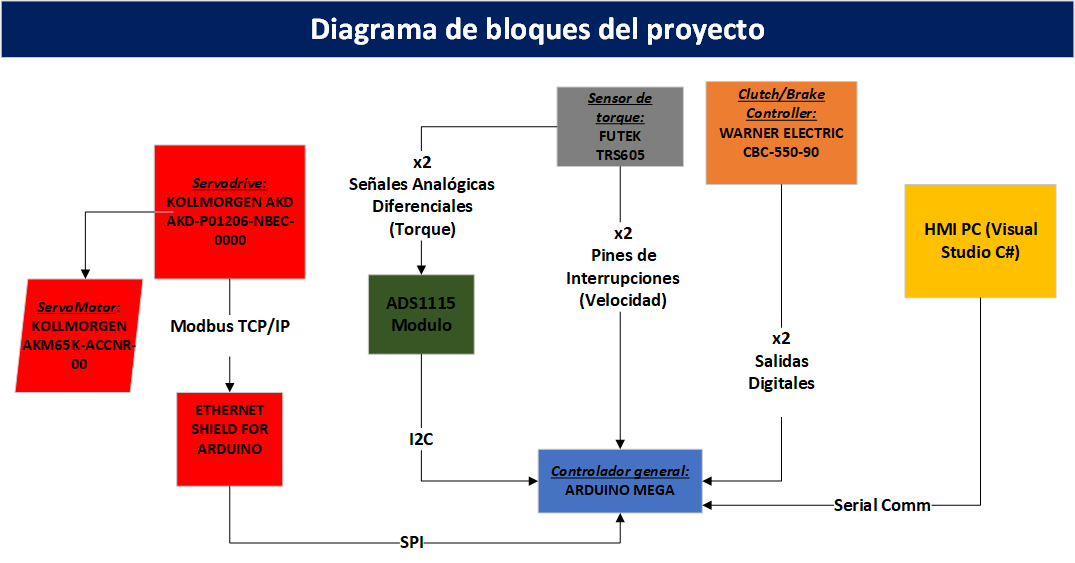
\includegraphics[scale=0.58]{bloques_diagram}
\caption{Diagrama de bloques del proyecto}
\end{figure}


\end{document}
